% Options for packages loaded elsewhere
% Options for packages loaded elsewhere
\PassOptionsToPackage{unicode}{hyperref}
\PassOptionsToPackage{hyphens}{url}
\PassOptionsToPackage{dvipsnames,svgnames,x11names}{xcolor}
%
\documentclass[
  letterpaper,
  DIV=11,
  numbers=noendperiod]{scrartcl}
\usepackage{xcolor}
\usepackage{amsmath,amssymb}
\setcounter{secnumdepth}{-\maxdimen} % remove section numbering
\usepackage{iftex}
\ifPDFTeX
  \usepackage[T1]{fontenc}
  \usepackage[utf8]{inputenc}
  \usepackage{textcomp} % provide euro and other symbols
\else % if luatex or xetex
  \usepackage{unicode-math} % this also loads fontspec
  \defaultfontfeatures{Scale=MatchLowercase}
  \defaultfontfeatures[\rmfamily]{Ligatures=TeX,Scale=1}
\fi
\usepackage{lmodern}
\ifPDFTeX\else
  % xetex/luatex font selection
\fi
% Use upquote if available, for straight quotes in verbatim environments
\IfFileExists{upquote.sty}{\usepackage{upquote}}{}
\IfFileExists{microtype.sty}{% use microtype if available
  \usepackage[]{microtype}
  \UseMicrotypeSet[protrusion]{basicmath} % disable protrusion for tt fonts
}{}
\makeatletter
\@ifundefined{KOMAClassName}{% if non-KOMA class
  \IfFileExists{parskip.sty}{%
    \usepackage{parskip}
  }{% else
    \setlength{\parindent}{0pt}
    \setlength{\parskip}{6pt plus 2pt minus 1pt}}
}{% if KOMA class
  \KOMAoptions{parskip=half}}
\makeatother
% Make \paragraph and \subparagraph free-standing
\makeatletter
\ifx\paragraph\undefined\else
  \let\oldparagraph\paragraph
  \renewcommand{\paragraph}{
    \@ifstar
      \xxxParagraphStar
      \xxxParagraphNoStar
  }
  \newcommand{\xxxParagraphStar}[1]{\oldparagraph*{#1}\mbox{}}
  \newcommand{\xxxParagraphNoStar}[1]{\oldparagraph{#1}\mbox{}}
\fi
\ifx\subparagraph\undefined\else
  \let\oldsubparagraph\subparagraph
  \renewcommand{\subparagraph}{
    \@ifstar
      \xxxSubParagraphStar
      \xxxSubParagraphNoStar
  }
  \newcommand{\xxxSubParagraphStar}[1]{\oldsubparagraph*{#1}\mbox{}}
  \newcommand{\xxxSubParagraphNoStar}[1]{\oldsubparagraph{#1}\mbox{}}
\fi
\makeatother

\usepackage{color}
\usepackage{fancyvrb}
\newcommand{\VerbBar}{|}
\newcommand{\VERB}{\Verb[commandchars=\\\{\}]}
\DefineVerbatimEnvironment{Highlighting}{Verbatim}{commandchars=\\\{\}}
% Add ',fontsize=\small' for more characters per line
\usepackage{framed}
\definecolor{shadecolor}{RGB}{241,243,245}
\newenvironment{Shaded}{\begin{snugshade}}{\end{snugshade}}
\newcommand{\AlertTok}[1]{\textcolor[rgb]{0.68,0.00,0.00}{#1}}
\newcommand{\AnnotationTok}[1]{\textcolor[rgb]{0.37,0.37,0.37}{#1}}
\newcommand{\AttributeTok}[1]{\textcolor[rgb]{0.40,0.45,0.13}{#1}}
\newcommand{\BaseNTok}[1]{\textcolor[rgb]{0.68,0.00,0.00}{#1}}
\newcommand{\BuiltInTok}[1]{\textcolor[rgb]{0.00,0.23,0.31}{#1}}
\newcommand{\CharTok}[1]{\textcolor[rgb]{0.13,0.47,0.30}{#1}}
\newcommand{\CommentTok}[1]{\textcolor[rgb]{0.37,0.37,0.37}{#1}}
\newcommand{\CommentVarTok}[1]{\textcolor[rgb]{0.37,0.37,0.37}{\textit{#1}}}
\newcommand{\ConstantTok}[1]{\textcolor[rgb]{0.56,0.35,0.01}{#1}}
\newcommand{\ControlFlowTok}[1]{\textcolor[rgb]{0.00,0.23,0.31}{\textbf{#1}}}
\newcommand{\DataTypeTok}[1]{\textcolor[rgb]{0.68,0.00,0.00}{#1}}
\newcommand{\DecValTok}[1]{\textcolor[rgb]{0.68,0.00,0.00}{#1}}
\newcommand{\DocumentationTok}[1]{\textcolor[rgb]{0.37,0.37,0.37}{\textit{#1}}}
\newcommand{\ErrorTok}[1]{\textcolor[rgb]{0.68,0.00,0.00}{#1}}
\newcommand{\ExtensionTok}[1]{\textcolor[rgb]{0.00,0.23,0.31}{#1}}
\newcommand{\FloatTok}[1]{\textcolor[rgb]{0.68,0.00,0.00}{#1}}
\newcommand{\FunctionTok}[1]{\textcolor[rgb]{0.28,0.35,0.67}{#1}}
\newcommand{\ImportTok}[1]{\textcolor[rgb]{0.00,0.46,0.62}{#1}}
\newcommand{\InformationTok}[1]{\textcolor[rgb]{0.37,0.37,0.37}{#1}}
\newcommand{\KeywordTok}[1]{\textcolor[rgb]{0.00,0.23,0.31}{\textbf{#1}}}
\newcommand{\NormalTok}[1]{\textcolor[rgb]{0.00,0.23,0.31}{#1}}
\newcommand{\OperatorTok}[1]{\textcolor[rgb]{0.37,0.37,0.37}{#1}}
\newcommand{\OtherTok}[1]{\textcolor[rgb]{0.00,0.23,0.31}{#1}}
\newcommand{\PreprocessorTok}[1]{\textcolor[rgb]{0.68,0.00,0.00}{#1}}
\newcommand{\RegionMarkerTok}[1]{\textcolor[rgb]{0.00,0.23,0.31}{#1}}
\newcommand{\SpecialCharTok}[1]{\textcolor[rgb]{0.37,0.37,0.37}{#1}}
\newcommand{\SpecialStringTok}[1]{\textcolor[rgb]{0.13,0.47,0.30}{#1}}
\newcommand{\StringTok}[1]{\textcolor[rgb]{0.13,0.47,0.30}{#1}}
\newcommand{\VariableTok}[1]{\textcolor[rgb]{0.07,0.07,0.07}{#1}}
\newcommand{\VerbatimStringTok}[1]{\textcolor[rgb]{0.13,0.47,0.30}{#1}}
\newcommand{\WarningTok}[1]{\textcolor[rgb]{0.37,0.37,0.37}{\textit{#1}}}

\usepackage{longtable,booktabs,array}
\usepackage{calc} % for calculating minipage widths
% Correct order of tables after \paragraph or \subparagraph
\usepackage{etoolbox}
\makeatletter
\patchcmd\longtable{\par}{\if@noskipsec\mbox{}\fi\par}{}{}
\makeatother
% Allow footnotes in longtable head/foot
\IfFileExists{footnotehyper.sty}{\usepackage{footnotehyper}}{\usepackage{footnote}}
\makesavenoteenv{longtable}
\usepackage{graphicx}
\makeatletter
\newsavebox\pandoc@box
\newcommand*\pandocbounded[1]{% scales image to fit in text height/width
  \sbox\pandoc@box{#1}%
  \Gscale@div\@tempa{\textheight}{\dimexpr\ht\pandoc@box+\dp\pandoc@box\relax}%
  \Gscale@div\@tempb{\linewidth}{\wd\pandoc@box}%
  \ifdim\@tempb\p@<\@tempa\p@\let\@tempa\@tempb\fi% select the smaller of both
  \ifdim\@tempa\p@<\p@\scalebox{\@tempa}{\usebox\pandoc@box}%
  \else\usebox{\pandoc@box}%
  \fi%
}
% Set default figure placement to htbp
\def\fps@figure{htbp}
\makeatother





\setlength{\emergencystretch}{3em} % prevent overfull lines

\providecommand{\tightlist}{%
  \setlength{\itemsep}{0pt}\setlength{\parskip}{0pt}}



 


\KOMAoption{captions}{tableheading}
\makeatletter
\@ifpackageloaded{caption}{}{\usepackage{caption}}
\AtBeginDocument{%
\ifdefined\contentsname
  \renewcommand*\contentsname{Table of contents}
\else
  \newcommand\contentsname{Table of contents}
\fi
\ifdefined\listfigurename
  \renewcommand*\listfigurename{List of Figures}
\else
  \newcommand\listfigurename{List of Figures}
\fi
\ifdefined\listtablename
  \renewcommand*\listtablename{List of Tables}
\else
  \newcommand\listtablename{List of Tables}
\fi
\ifdefined\figurename
  \renewcommand*\figurename{Figure}
\else
  \newcommand\figurename{Figure}
\fi
\ifdefined\tablename
  \renewcommand*\tablename{Table}
\else
  \newcommand\tablename{Table}
\fi
}
\@ifpackageloaded{float}{}{\usepackage{float}}
\floatstyle{ruled}
\@ifundefined{c@chapter}{\newfloat{codelisting}{h}{lop}}{\newfloat{codelisting}{h}{lop}[chapter]}
\floatname{codelisting}{Listing}
\newcommand*\listoflistings{\listof{codelisting}{List of Listings}}
\makeatother
\makeatletter
\makeatother
\makeatletter
\@ifpackageloaded{caption}{}{\usepackage{caption}}
\@ifpackageloaded{subcaption}{}{\usepackage{subcaption}}
\makeatother
\usepackage{bookmark}
\IfFileExists{xurl.sty}{\usepackage{xurl}}{} % add URL line breaks if available
\urlstyle{same}
\hypersetup{
  pdftitle={Welcome to CSI 4106!},
  colorlinks=true,
  linkcolor={blue},
  filecolor={Maroon},
  citecolor={Blue},
  urlcolor={Blue},
  pdfcreator={LaTeX via pandoc}}


\title{Welcome to CSI 4106!}
\author{}
\date{}
\begin{document}
\maketitle


CSI 4106 - Fall 2025

Marcel Turcotte\\
Version: Sep 2, 2025 18:35

\section{Preamble}\label{preamble}

\subsection{Message of the day (MOTD)}\label{message-of-the-day-motd}

\pandocbounded{\includegraphics[keepaspectratio]{slides_files/mediabag/portrait-of-joelle-p.webp}}

\begin{itemize}
\tightlist
\item
  2025-08 -- Chief AI Officer, \href{https://cohere.com}{Cohere}
\item
  2023-03 -- 2025-05 VP AI Research, Meta
\item
  2017-05 -- 2023-02 Director, Facebook Artificial Intelligence Research
  (FAIR), Montréal
\item
  2004-08 -- Professor, McGill University
\end{itemize}

\href{https://www.theglobeandmail.com/business/article-cohere-fundraising-former-meta-executive-joelle-pineau-ai/}{Cohere
raises US\$500-million, hires former Meta AI expert Joelle Pineau}, Joe
Castaldo, The Globe and Mail, 2025-08-14.

\href{https://en.wikipedia.org/wiki/Joëlle_Pineau}{Joëlle\_Pineau}, a
distinguished Canadian computer scientist, was born in Ottawa and has
had an exemplary career in the field of artificial intelligence
research. She previously held the position of Vice President of AI
Research at Meta and served as the Director of Facebook Artificial
Intelligence Research (FAIR) in Montréal. Currently, she is the Chief AI
Officer at Cohere.

Cohere, a Canadian AI company, is dedicated to the development of
advanced natural language processing (NLP) technologies aimed at
equipping businesses with state-of-the-art language models. Two of its
cofounders, Aidan Gomez and Nick Frosst, previously conducted research
at Google Brain. They are also co-authors of the landmark paper
``\href{https://arxiv.org/abs/1706.03762}{Attention is All You Need},''
which introduced the transformer architecture, a key advancement in
machine learning. The paper has 192,363 citations according to Google
Scholar.

\begin{center}\rule{0.5\linewidth}{0.5pt}\end{center}

\url{https://youtu.be/Sq1QZB5baNw}

The presentation includes four videos, but we will only watch one. These
videos were chosen for their science fiction aspect and their use of
generative AI.

Figure's approach is markedly different from earlier methods. The latter
often relied on separate modules to solve different problems. For
example, a robot would use a planning algorithm to find an optimal path,
and the reasoning was heavily scripted (``on rails''), thus limiting
tasks and learning capabilities.

Here, we see an end-to-end approach based on neural networks. Deep
learning aims to produce flexible, general, and capable learning
systems. Inspired by large language models (LLMs), we are now observing
the development of large action models (LAMs).

The videos on the new models from Google DeepMind are equally
impressive.

How do you feel about these developments?

\begin{center}\rule{0.5\linewidth}{0.5pt}\end{center}

\url{https://youtu.be/Z3yQHYNXPws}

\begin{center}\rule{0.5\linewidth}{0.5pt}\end{center}

\url{https://youtu.be/UIZAiXYceBI}

\begin{center}\rule{0.5\linewidth}{0.5pt}\end{center}

\url{https://youtu.be/nXVvvRhiGjI}

\subsection{Learning objectives}\label{learning-objectives}

\begin{itemize}
\tightlist
\item
  \textbf{Clarify} the proposition
\item
  \textbf{Discuss} the syllabus
\item
  \textbf{Articulate} the expectations
\item
  \textbf{Explore} the various definitions of ``artificial
  intelligence''
\end{itemize}

I want to clarify my proposal. I have chosen a specific approach to
introduce the concepts and I would like to explain the reasons for this
choice.

After presenting the course outline and expectations, we will discuss
the different definitions of artificial intelligence.

\section{Proposition}\label{proposition}

\subsection{Course overview}\label{course-overview}

\begin{quote}
\textbf{Calendar description}

The roots and scope of Artificial Intelligence. Knowledge and knowledge
representation. Search, informed search, adversarial search. Deduction
and reasoning. Uncertainty in Artificial Intelligence. Introduction to
Natural Language Processing. Elements of planning. Basics of Machine
Learning.
\end{quote}

Here is the official course description. At the end of this
presentation, you will find the Python code I used to produce this audio
clip.

This course description dates back several years, placing machine
learning at the end of the list.

\subsection{Aims: Deep learning early}\label{aims-deep-learning-early}

\begin{quote}
** (Legg and Hutter 2007)**

To the larger community of computer science and information technology,
\textbf{AI} is usually \textbf{identified by the techniques grown from
it}, which at \textbf{different periods} may include \textbf{theorem
proving}, \textbf{heuristic search}, \textbf{game playing},
\textbf{expert systems}, \textbf{neural networks}, \textbf{Bayesian
networks}, \textbf{data mining}, \textbf{agents}, and recently,
\textbf{deep learning}.
\end{quote}

\begin{itemize}
\tightlist
\item
  \textbf{Deep learning} is so dominant that I have chosen to structure
  everything around it
\end{itemize}

\subsection{What does it means?}\label{what-does-it-means}

\textbf{Good Old-Fashioned AI} (\textbf{GOFAI}) relied on
\textbf{hand-crafted knowledge engineering}, but it has been largely
displaced by \textbf{machine learning} due to the increased availability
of data, computing resources, and new algorithms.

. . .

\textbf{Deep learning} has significantly impacted various domains,
including natural language processing, robotics, and computer vision.

. . .

However, deep learning has current \textbf{limitations}, particularly in
\textbf{reasoning}, where symbolic AI excels and could potentially offer
valuable insights.

\subsection{But also}\label{but-also}

\pandocbounded{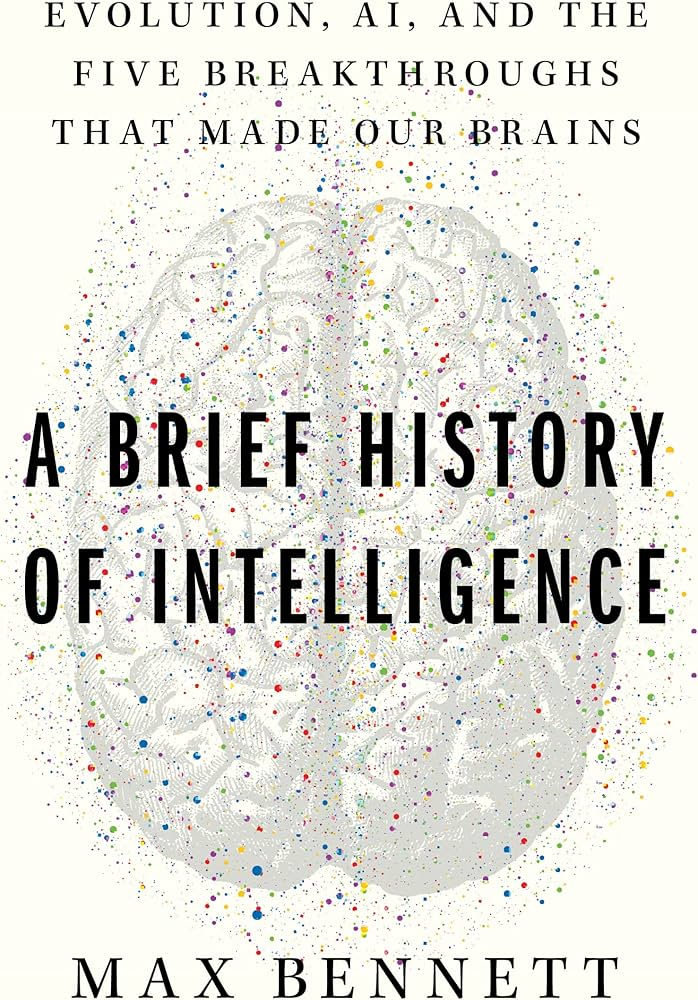
\includegraphics[keepaspectratio]{slides_files/mediabag/81xA5147ATL._AC_UF10.jpg}}

\begin{itemize}
\tightlist
\item
  In \textbf{\href{https://www.abriefhistoryofintelligence.com/book}{A
  Brief History of Intelligence}} (Bennett 2023), Max Bennett discusses
  \textbf{significant milestones in the evolution of human intelligence}
  and draws parallels to advancements in artificial intelligence (AI).
\item
  Learning itself represents one of the earliest and most extensively
  understood milestones in the evolution of intelligence.
\end{itemize}

Curiously, the development of AI has been largely influenced by logical
approaches (symbolic AI). The development of AI has been strongly marked
by intellectual currents rooted in philosophy and mathematics, rather
than in biology and its evolution. Reasoning in philosophy and
mathematics relies on complex cognitive functions, perhaps less well
understood and having evolved later.

Learning itself represents one of the first and most widely understood
steps in the evolution of intelligence.

It would have been logical to approach the study of intelligence by
progressing from simpler forms to more complex ones.

\subsection{Aims: Applied}\label{aims-applied}

\begin{quote}
** Andrew Ng,
\href{https://info.deeplearning.ai/autonomous-coding-agents-instability-at-stability-ai-mamba-mania-what-users-do-with-genai-2}{The
Batch, April 10, 2024}**

Many software developers worry that \textbf{large language models} will
make \textbf{human coders obsolete.} We doubt that AI will replace
coders, but we believe that \textbf{coders who use AI will replace those
who don't}.
\end{quote}

\begin{itemize}
\tightlist
\item
  Whenever possible, concepts will be introduced with code.
\end{itemize}

\subsection{Aims: Academic rigour}\label{aims-academic-rigour}

In pursuing clarity and accessibility, this course aims to strike a
balance between \textbf{informal discourse} and the \textbf{precision}
required for academic rigour. The objective is for learners to not only
grasp but also \textbf{apply}, \textbf{evaluate}, and \textbf{critically
analyze} the concepts discussed throughout the course.

\section{Syllabus}\label{syllabus}

\subsection{Course information}\label{course-information}

\subsubsection{Web sites}\label{web-sites}

\begin{itemize}
\tightlist
\item
  \href{https://turcotte.xyz/teaching/csi-4106}{turcotte.xyz/teaching/csi-4106}
\item
  \href{https://uottawa.brightspace.ca}{uottawa.brightspace.ca}
\end{itemize}

\subsubsection{Schedule}\label{schedule}

\begin{itemize}
\tightlist
\item
  \textbf{Lectures:} Mon 13:00-14:20 and Wed 11:30-12:50 CRX C240
\item
  \textbf{Office hours:} Mon 15:00-16:20 STE 5106
\item
  \textbf{Official schedule:}
  \href{https://www.uottawa.ca/course-timetable}{www.uottawa.ca/course-timetable}
\end{itemize}

\subsubsection{Grading}\label{grading}

\begin{longtable}[]{@{}ll@{}}
\toprule\noalign{}
Category & Percentage \\
\midrule\noalign{}
\endhead
\bottomrule\noalign{}
\endlastfoot
Assignments & 40\% (4 x 10\%) \\
Quiz & 20\% \\
Final examination & 40\% \\
\end{longtable}

\subsubsection{Reading material}\label{reading-material}

I will draw upon insights from the two comprehensive textbooks listed
below, as well as relevant scientific publications. Additionally, all
sources of information will be cited. For most people, I expect that my
lecture notes will be sufficient.

\begin{itemize}
\tightlist
\item
  Russell, S., \& Norvig, P. (2020).
  \href{https://aima.cs.berkeley.edu/}{\emph{Artificial Intelligence: A
  Modern Approach}} (4th ed.). Pearson.
\item
  Poole, D.L., \& Mackworth, A.K. (2023)
  \href{https://artint.info}{\emph{Artificial Intelligence: Foundations
  of Computational Agents}} (3rd ed.). Cambridge University Press.
  (Freely available online in
  \href{https://artint.info/3e/html/ArtInt3e.html}{HTML format})
\end{itemize}

The \href{https://www.bkstr.com/ottawastore/home}{Campus Store} has
ordered a small number of copies of these books, for those interested.

We do not closely adhere to the framework proposed by (Russell and
Norvig 2020) and (Poole and Mackworth 2023). Specifically, while these
textbooks use the concept of an intelligent agent as a central theme,
fields such as machine learning (ML), natural language processing (NLP),
and vision operate as distinct communities. In these communities,
problems are typically not framed in terms of agents.

There are two websites to use. On my personal site, you will find
presentations and code examples. On Brightspace, you will submit your
assignments and participate in discussion groups.

During class, visit my personal website. There, you can review the
complete syllabus, the course schedule, information about the team, and
the brief biography of the instructor.

\subsection{Beta testers}\label{beta-testers}

This will be my second iteration of this content. Your help identifying
what works and what doesn't will be most appreciated.

\subsection{Warnings}\label{warnings}

CSI 4106 is an introductory course on artificial intelligence, offering
a brief overview of various topics within this broad field. \textbf{Each
topic covered could be explored in much greater depth through one or
more graduate-level courses.} The primary objective of CSI 4106 is to
provide students with a foundational understanding of the core areas
that constitute artificial intelligence.

. . .

Overlaps with other courses are inevitable, but I will do my best to
keep it at a minimum.

. . .

This is not a course on the impact of AI on society, including ethics,
fairness, trust and safety.

This warning is actually for myself. These are topics I am passionate
about, and I would love to share everything I know with you. However,
that is obviously not possible. Generally, I will try to focus on a
small number of approaches to thoroughly understand the subjects, rather
than adopting an exhaustive approach.

\section{Setting the Stage: AI, Deep Learning, and Diverging Views on
Intelligence.}\label{setting-the-stage-ai-deep-learning-and-diverging-views-on-intelligence.}

\subsection{AI, ML, DL}\label{ai-ml-dl}

\pandocbounded{\includegraphics[keepaspectratio]{slides_files/mediabag/1855px-AI-ML-DL.svg.png}}

\textbf{Attribution:} Avimanyu786SVG version: Tukijaaliwa,
\href{https://creativecommons.org/licenses/by-sa/4.0}{CC BY-SA 4.0},
visited 2024-06-18.

Deep learning is so prevalent today that some people might confuse it
with artificial intelligence. As the figure shows, deep learning is one
of many techniques used in machine learning. Machine learning, in turn,
is one of several disciplines within artificial intelligence. Other AI
disciplines include knowledge representation, reasoning and planning,
natural language processing, computer vision, and robotics.

By the end of this course, this distinction should be very clear.

\subsection{Schools of thought}\label{schools-of-thought}

\begin{itemize}
\tightlist
\item
  \textbf{Symbolic AI} (includes approaches based on logic)
\item
  \textbf{Connectionists} (mostly neural networks)
\end{itemize}

Long seen as mutually exclusive

At the outset of this course, it is important to recognize that two main
schools of thought exist in AI: \textbf{symbolic AI} and
\textbf{connectionism}. Initially, the symbolic approach was dominant in
the field of AI, but today, the connectionist approach prevails.

\subsection{Towers of Hanoi}\label{towers-of-hanoi}

(for your information only)

\url{https://youtu.be/PGuRmqpr6Oo}

\textbf{See also:} Binary, Hanoi and Sierpinski,
\href{https://www.youtube.com/watch?v=2SUvWfNJSsM}{Part 1} and
\href{https://www.youtube.com/watch?v=bdMfjfT0lKk}{Part 2}, by
\href{https://www.youtube.com/@3blue1brown}{3Blue1Brown}.

\subsection{Symbolic AI (Planning)}\label{symbolic-ai-planning}

\subsubsection{Problem}\label{problem}

The \textbf{Towers of Hanoi} is a puzzle that consists of \textbf{three
pegs} and \textbf{a number of disks of different sizes}. The puzzle
\textbf{starts} with all the \textbf{disks stacked in decreasing size on
one peg}, and the \textbf{goal is to move the entire stack to another
peg}, following these rules:

\begin{enumerate}
\def\labelenumi{\arabic{enumi}.}
\tightlist
\item
  \textbf{Only one disk} can be moved at a time.
\item
  A disk can only be placed \textbf{on top of a larger disk} or
  \textbf{on an empty peg}.
\end{enumerate}

\subsubsection{Rules}\label{rules}

\begin{Shaded}
\begin{Highlighting}[]
\DataTypeTok{Action} \DataTypeTok{Move}\NormalTok{(}\DataTypeTok{X}\KeywordTok{,}\DataTypeTok{Y}\KeywordTok{,}\DataTypeTok{Z}\NormalTok{)}\FunctionTok{:}
    \DataTypeTok{Preconditions} \KeywordTok{=} \KeywordTok{\{}\DataTypeTok{Clear}\NormalTok{(}\DataTypeTok{X}\NormalTok{)}\KeywordTok{,} \DataTypeTok{On}\NormalTok{(}\DataTypeTok{X}\KeywordTok{,}\DataTypeTok{Y}\NormalTok{)}\KeywordTok{,} \DataTypeTok{Clear}\NormalTok{(}\DataTypeTok{Z}\NormalTok{)}\KeywordTok{,} \DataTypeTok{Smaller}\NormalTok{(}\DataTypeTok{X}\KeywordTok{,}\DataTypeTok{Z}\NormalTok{)}\KeywordTok{\};}
    \DataTypeTok{Effects} \KeywordTok{=} \KeywordTok{\{}\FunctionTok{{-}}\DataTypeTok{On}\NormalTok{(}\DataTypeTok{X}\KeywordTok{,}\DataTypeTok{Y}\NormalTok{)}\KeywordTok{,} \DataTypeTok{Clear}\NormalTok{(}\DataTypeTok{Y}\NormalTok{)}\KeywordTok{,} \DataTypeTok{On}\NormalTok{(}\DataTypeTok{X}\KeywordTok{,}\DataTypeTok{Z}\NormalTok{)}\KeywordTok{,} \FunctionTok{{-}}\DataTypeTok{Clear}\NormalTok{(}\DataTypeTok{Z}\NormalTok{)}\KeywordTok{\};}
\end{Highlighting}
\end{Shaded}

\subsubsection{Start}\label{start}

\texttt{D1,\ D2,\ D3,\ P1,\ P2,\ P3} are \textbf{symbols}, where
\texttt{D1}, \texttt{D2}, and \texttt{D3} are disks, and \texttt{P1},
\texttt{P2}, and \texttt{P3} are pegs.

\begin{Shaded}
\begin{Highlighting}[]
\DataTypeTok{On}\NormalTok{(}\DataTypeTok{D1}\KeywordTok{,} \DataTypeTok{D2}\NormalTok{)}\KeywordTok{,} \DataTypeTok{On}\NormalTok{(}\DataTypeTok{D2}\KeywordTok{,} \DataTypeTok{D3}\NormalTok{)}\KeywordTok{,} \DataTypeTok{On}\NormalTok{(}\DataTypeTok{D3}\KeywordTok{,} \DataTypeTok{P1}\NormalTok{)}\KeywordTok{,}
\NormalTok{clear(}\DataTypeTok{D1}\NormalTok{)}\KeywordTok{,}\NormalTok{ clear(}\DataTypeTok{P2}\NormalTok{)}\KeywordTok{,}\NormalTok{ clear(}\DataTypeTok{P3}\NormalTok{)}\KeywordTok{,}
\DataTypeTok{Smaller}\NormalTok{(}\DataTypeTok{D1}\KeywordTok{,} \DataTypeTok{D2}\NormalTok{)}\KeywordTok{,} \DataTypeTok{Smaller}\NormalTok{(}\DataTypeTok{D1}\KeywordTok{,} \DataTypeTok{D3}\NormalTok{)}\KeywordTok{,} \DataTypeTok{Smaller}\NormalTok{(}\DataTypeTok{D2}\KeywordTok{,} \DataTypeTok{D3}\NormalTok{)}\KeywordTok{,}
\DataTypeTok{Smaller}\NormalTok{(}\DataTypeTok{D1}\KeywordTok{,} \DataTypeTok{P1}\NormalTok{)}\KeywordTok{,} \DataTypeTok{Smaller}\NormalTok{(}\DataTypeTok{D1}\KeywordTok{,} \DataTypeTok{P2}\NormalTok{)}\KeywordTok{,} \DataTypeTok{Smaller}\NormalTok{(}\DataTypeTok{D1}\KeywordTok{,} \DataTypeTok{P3}\NormalTok{)}\KeywordTok{,}
\DataTypeTok{Smaller}\NormalTok{(}\DataTypeTok{D2}\KeywordTok{,} \DataTypeTok{P1}\NormalTok{)}\KeywordTok{,} \DataTypeTok{Smaller}\NormalTok{(}\DataTypeTok{D2}\KeywordTok{,} \DataTypeTok{P2}\NormalTok{)}\KeywordTok{,} \DataTypeTok{Smaller}\NormalTok{(}\DataTypeTok{D2}\KeywordTok{,} \DataTypeTok{P3}\NormalTok{)}\KeywordTok{,}
\DataTypeTok{Smaller}\NormalTok{(}\DataTypeTok{D3}\KeywordTok{,} \DataTypeTok{P1}\NormalTok{)}\KeywordTok{,} \DataTypeTok{Smaller}\NormalTok{(}\DataTypeTok{D3}\KeywordTok{,} \DataTypeTok{P2}\NormalTok{)}\KeywordTok{,} \DataTypeTok{Smaller}\NormalTok{(}\DataTypeTok{D3}\KeywordTok{,} \DataTypeTok{P3}\NormalTok{)}\KeywordTok{.}
\end{Highlighting}
\end{Shaded}

\subsubsection{Goal}\label{goal}

\begin{Shaded}
\begin{Highlighting}[]
\DataTypeTok{On}\NormalTok{(}\DataTypeTok{D1}\KeywordTok{,} \DataTypeTok{D2}\NormalTok{)}\KeywordTok{,} \DataTypeTok{On}\NormalTok{(}\DataTypeTok{D2}\KeywordTok{,} \DataTypeTok{D3}\NormalTok{)}\KeywordTok{,} \DataTypeTok{On}\NormalTok{(}\DataTypeTok{D3}\KeywordTok{,} \DataTypeTok{P3}\NormalTok{)}\KeywordTok{.}
\end{Highlighting}
\end{Shaded}

\subsubsection{Solution}\label{solution}

\begin{Shaded}
\begin{Highlighting}[]
\DataTypeTok{Move}\NormalTok{(}\DataTypeTok{D1}\KeywordTok{,} \DataTypeTok{P1}\KeywordTok{,} \DataTypeTok{P3}\NormalTok{)}
\DataTypeTok{Move}\NormalTok{(}\DataTypeTok{D2}\KeywordTok{,} \DataTypeTok{P1}\KeywordTok{,} \DataTypeTok{P2}\NormalTok{)}
\DataTypeTok{Move}\NormalTok{(}\DataTypeTok{D1}\KeywordTok{,} \DataTypeTok{P3}\KeywordTok{,} \DataTypeTok{P2}\NormalTok{)}
\DataTypeTok{Move}\NormalTok{(}\DataTypeTok{D3}\KeywordTok{,} \DataTypeTok{P1}\KeywordTok{,} \DataTypeTok{P3}\NormalTok{)}
\DataTypeTok{Move}\NormalTok{(}\DataTypeTok{D1}\KeywordTok{,} \DataTypeTok{P2}\KeywordTok{,} \DataTypeTok{P1}\NormalTok{)}
\DataTypeTok{Move}\NormalTok{(}\DataTypeTok{D2}\KeywordTok{,} \DataTypeTok{P2}\KeywordTok{,} \DataTypeTok{P3}\NormalTok{)}
\DataTypeTok{Move}\NormalTok{(}\DataTypeTok{D1}\KeywordTok{,} \DataTypeTok{P1}\KeywordTok{,} \DataTypeTok{P3}\NormalTok{)}
\end{Highlighting}
\end{Shaded}

\textbf{STRIPS (Stanford Research Institute Problem Solver, 1971)} is a
\textbf{classical AI planning system} that represents problems in terms
of:

\begin{itemize}
\tightlist
\item
  \textbf{States}: sets of logical predicates describing the world.
\item
  \textbf{Operators (Actions)}: defined by

  \begin{itemize}
  \tightlist
  \item
    \emph{Preconditions}: predicates that must be true to apply the
    action,
  \item
    \emph{Add list}: predicates made true after execution,
  \item
    \emph{Delete list}: predicates made false after execution.
  \end{itemize}
\item
  \textbf{Goal}: a set of predicates to be achieved.
\end{itemize}

A plan is found by applying actions to transform the initial state into
a goal state, updating the world via the add/delete lists.

These methods will be examined in depth starting from Lecture 16,
focused on search methods, and Lecture 22, which will cover formal
reasoning.

\subsection{Symbolic AI (Kinship)}\label{symbolic-ai-kinship}

\subsubsection{Problem}\label{problem-1}

Given a few \textbf{facts} about who is parent of whom
(\textbf{symbols}) and a handful of \textbf{Horn-clause rules}, infer
new relations (e.g., \textbf{ancestor}, \textbf{siblings},
\textbf{grandparent}) by \emph{logical deduction}.

\subsubsection{Rules}\label{rules-1}

\begin{Shaded}
\begin{Highlighting}[]
\NormalTok{father(}\DataTypeTok{F}\KeywordTok{,}\DataTypeTok{C}\NormalTok{) }\KeywordTok{:{-}}\NormalTok{ male(}\DataTypeTok{F}\NormalTok{)}\KeywordTok{,}\NormalTok{ parent(}\DataTypeTok{F}\KeywordTok{,}\DataTypeTok{C}\NormalTok{)}\KeywordTok{.}
\NormalTok{mother(}\DataTypeTok{M}\KeywordTok{,}\DataTypeTok{C}\NormalTok{) }\KeywordTok{:{-}}\NormalTok{ female(}\DataTypeTok{M}\NormalTok{)}\KeywordTok{,}\NormalTok{ parent(}\DataTypeTok{M}\KeywordTok{,}\DataTypeTok{C}\NormalTok{)}\KeywordTok{.}

\NormalTok{sibling(}\DataTypeTok{X}\KeywordTok{,}\DataTypeTok{Y}\NormalTok{) }\KeywordTok{:{-}}\NormalTok{ parent(}\DataTypeTok{P}\KeywordTok{,}\DataTypeTok{X}\NormalTok{)}\KeywordTok{,}\NormalTok{ parent(}\DataTypeTok{P}\KeywordTok{,}\DataTypeTok{Y}\NormalTok{)}\KeywordTok{,} \DataTypeTok{X} \KeywordTok{\textbackslash{}=} \DataTypeTok{Y}\KeywordTok{.}

\NormalTok{grandparent(}\DataTypeTok{G}\KeywordTok{,}\DataTypeTok{C}\NormalTok{) }\KeywordTok{:{-}}\NormalTok{ parent(}\DataTypeTok{G}\KeywordTok{,}\DataTypeTok{P}\NormalTok{)}\KeywordTok{,}\NormalTok{ parent(}\DataTypeTok{P}\KeywordTok{,}\DataTypeTok{C}\NormalTok{)}\KeywordTok{.}

\NormalTok{ancestor(}\DataTypeTok{A}\KeywordTok{,}\DataTypeTok{D}\NormalTok{) }\KeywordTok{:{-}}\NormalTok{ parent(}\DataTypeTok{A}\KeywordTok{,}\DataTypeTok{D}\NormalTok{)}\KeywordTok{.}
\NormalTok{ancestor(}\DataTypeTok{A}\KeywordTok{,}\DataTypeTok{D}\NormalTok{) }\KeywordTok{:{-}}\NormalTok{ parent(}\DataTypeTok{A}\KeywordTok{,}\DataTypeTok{X}\NormalTok{)}\KeywordTok{,}\NormalTok{ ancestor(}\DataTypeTok{X}\KeywordTok{,}\DataTypeTok{D}\NormalTok{)}\KeywordTok{.}
\end{Highlighting}
\end{Shaded}

\subsubsection{Facts}\label{facts}

\begin{Shaded}
\begin{Highlighting}[]
\CommentTok{\% facts/symbols}

\NormalTok{male(alan)}\KeywordTok{.}\NormalTok{  female(brenda)}\KeywordTok{.}
\NormalTok{male(chris)}\KeywordTok{.}\NormalTok{ female(dina)}\KeywordTok{.}
\NormalTok{male(eli)}\KeywordTok{.}\NormalTok{   female(fiona)}\KeywordTok{.}

\NormalTok{parent(alan}\KeywordTok{,}\NormalTok{ chris)}\KeywordTok{.}
\NormalTok{parent(brenda}\KeywordTok{,}\NormalTok{ chris)}\KeywordTok{.}
\NormalTok{parent(chris}\KeywordTok{,}\NormalTok{ dina)}\KeywordTok{.}
\NormalTok{parent(dina}\KeywordTok{,}\NormalTok{ eli)}\KeywordTok{.}
\NormalTok{parent(dina}\KeywordTok{,}\NormalTok{ fiona)}\KeywordTok{.}
\end{Highlighting}
\end{Shaded}

\subsubsection{Query}\label{query}

\begin{Shaded}
\begin{Highlighting}[]
\FunctionTok{?{-}}\NormalTok{ grandparent(}\DataTypeTok{G}\KeywordTok{,}\NormalTok{ dina)}\KeywordTok{.}
\CommentTok{\% Expected: G = alan ; G = brenda.}

\FunctionTok{?{-}}\NormalTok{ ancestor(}\DataTypeTok{A}\KeywordTok{,}\NormalTok{ fiona)}\KeywordTok{.}
\CommentTok{\% Expected: A = dina ; A = alan ; A = brenda ; A = chris ;}

\FunctionTok{?{-}}\NormalTok{ sibling(eli}\KeywordTok{,}\NormalTok{ fiona)}\KeywordTok{.}
\CommentTok{\% Expected: true.}
\end{Highlighting}
\end{Shaded}

The preceding example demonstrates the application of logic programming,
specifically Prolog, to articulate relationships between entities.

\begin{itemize}
\tightlist
\item
  \textbf{Clear separation} of knowledge (facts) and reasoning (rules).
\item
  \textbf{Explanations}: Prolog's proof trees make deductions
  inspectable.
\item
  \textbf{Recursion} illustrates expressive power (e.g., ancestor/2).
\end{itemize}

\subsection{Symbolic AI
(Prerequisites)}\label{symbolic-ai-prerequisites}

\subsubsection{Problem}\label{problem-2}

Given \textbf{course prerequisites} and a student's \textbf{completed}
set, infer which courses they \textbf{can take next}. This shows
\emph{symbolic constraint reasoning}.

\subsubsection{Rules}\label{rules-2}

\begin{Shaded}
\begin{Highlighting}[]
\NormalTok{all\_prereqs\_met(}\DataTypeTok{Student}\KeywordTok{,} \DataTypeTok{Course}\NormalTok{) }\KeywordTok{:{-}}
    \KeywordTok{\textbackslash{}+}\NormalTok{ (prereq(}\DataTypeTok{Course}\KeywordTok{,} \DataTypeTok{P}\NormalTok{)}\KeywordTok{,} \KeywordTok{\textbackslash{}+}\NormalTok{ completed(}\DataTypeTok{Student}\KeywordTok{,} \DataTypeTok{P}\NormalTok{))}\KeywordTok{.}

\NormalTok{can\_take(}\DataTypeTok{Student}\KeywordTok{,} \DataTypeTok{Course}\NormalTok{) }\KeywordTok{:{-}}
\NormalTok{    all\_prereqs\_met(}\DataTypeTok{Student}\KeywordTok{,} \DataTypeTok{Course}\NormalTok{)}\KeywordTok{,}
    \KeywordTok{\textbackslash{}+}\NormalTok{ completed(}\DataTypeTok{Student}\KeywordTok{,} \DataTypeTok{Course}\NormalTok{)}\KeywordTok{.}
\end{Highlighting}
\end{Shaded}

\subsubsection{Courses}\label{courses}

\begin{Shaded}
\begin{Highlighting}[]
\CommentTok{\% {-}{-}{-} Course graph (facts, symbols) {-}{-}{-}}

\NormalTok{prereq(csi2120}\KeywordTok{,}\NormalTok{ csi2110)}\KeywordTok{.}
\NormalTok{prereq(csi2110}\KeywordTok{,}\NormalTok{ iti1121)}\KeywordTok{.}
\NormalTok{prereq(csi2110}\KeywordTok{,}\NormalTok{ mat1338)}\KeywordTok{.}
\NormalTok{prereq(iti1121}\KeywordTok{,}\NormalTok{ iti1120)}\KeywordTok{.}
\end{Highlighting}
\end{Shaded}

\subsubsection{Students}\label{students}

\begin{Shaded}
\begin{Highlighting}[]
\CommentTok{\% {-}{-}{-} Student record (facts, symbols) {-}{-}{-}}

\NormalTok{completed(alex}\KeywordTok{,}\NormalTok{ iti1121)}\KeywordTok{.}
\NormalTok{completed(alex}\KeywordTok{,}\NormalTok{ iti1120)}\KeywordTok{.}
\NormalTok{completed(alex}\KeywordTok{,}\NormalTok{ mat1338)}\KeywordTok{.}
\end{Highlighting}
\end{Shaded}

\subsubsection{Query}\label{query-1}

\begin{Shaded}
\begin{Highlighting}[]
\FunctionTok{?{-}}\NormalTok{ can\_take(alex}\KeywordTok{,}\NormalTok{ csi2110)}\KeywordTok{.}
\CommentTok{\% true}

\FunctionTok{?{-}}\NormalTok{ can\_take(alex}\KeywordTok{,}\NormalTok{ csi2120)}\KeywordTok{.}
\CommentTok{\% false}

\FunctionTok{?{-}}\NormalTok{ can\_take(alex}\KeywordTok{,}\NormalTok{ iti1121)}\KeywordTok{.}
\CommentTok{\% false}

\FunctionTok{?{-}}\NormalTok{ all\_prereqs\_met(alex}\KeywordTok{,}\NormalTok{ csi2110)}\KeywordTok{.}
\CommentTok{\% true}
\end{Highlighting}
\end{Shaded}

Another example using logic programming (Prolog).

\begin{itemize}
\tightlist
\item
  Shows \textbf{constraint satisfaction} and \textbf{closed-world
  negation}.
\item
  Easy to extend with electives, co-requisites, or anti-requisites.
\item
  Produces \textbf{auditable recommendations} (why/why not).
\end{itemize}

Negation as failure, which is represented as \texttt{\textbackslash{}+}
(backslash-plus), Prolog.

\begin{itemize}
\tightlist
\item
  \texttt{\textbackslash{}+\ Goal} succeeds if \texttt{Goal} cannot be
  proven.
\item
  Semantics: \textbf{closed-world assumption} --- if it's not in the
  knowledge base, we assume it's false.
\end{itemize}

The rule

\begin{Shaded}
\begin{Highlighting}[]
\NormalTok{all\_prereqs\_met(Student, Course) :{-}}
\NormalTok{    \textbackslash{}+ (prereq(Course, P), \textbackslash{}+ completed(Student, P)).}
\end{Highlighting}
\end{Shaded}

reads as:

\begin{quote}
``\texttt{all\_prereqs\_met(Student,\ Course)} holds \textbf{if there
does not exist} a prerequisite \texttt{P} of \texttt{Course} such that
\texttt{Student} has not completed \texttt{P}.''
\end{quote}

Or, more naturally:

\begin{quote}
``A student has met all the prerequisites for a course when every course
that is listed as a prerequisite has already been completed by that
student.''
\end{quote}

\subsection{Symbolic AI}\label{symbolic-ai}

\begin{itemize}
\tightlist
\item
  ``Their founding tenet held that \textbf{knowledge} can be represented
  by a \textbf{set of rules}, and computer programs can use
  \textbf{logic} to manipulate that knowledge.'' (Strickland 2021)
\item
  ``Researchers developing symbolic AI set out to \textbf{explicitly
  teach computers} about the world.'' (Strickland 2021)
\item
  ``(\(\ldots\)) a \textbf{physical symbol system} has the
  \textbf{necessary} and \textbf{sufficient} means for \textbf{general
  intelligent action}.'' (Newell and Simon 1976)
\end{itemize}

Note the importance of the word ``explicitly'' in this statement. It is
not about providing examples to the computer, but rather about
describing human knowledge using logic.

The researchers of the time were convinced that the symbolic approach
was the key to success.

\subsection{Symbolic AI}\label{symbolic-ai-1}

\begin{itemize}
\tightlist
\item
  What were the \textbf{primary challenges} associated with
  \textbf{symbolic AI}?
\end{itemize}

\subsection{Connectionist}\label{connectionist}

Inspired by biology, \textbf{artificial neural networks} (\textbf{ANNs})
are computational models designed to \textbf{mimic the human brain's
network of neurons}. They consist of layers of \textbf{interconnected
nodes (neurons)}, each \textbf{connection} having an associated
\textbf{weight}.

. . .

ANNs process input data through these weighted connections, and
\textbf{learning} occurs by \textbf{adjusting the weights} based on
\textbf{errors} in the \textbf{training data}.

\textbf{See:}
\href{https://playground.tensorflow.org}{playground.tensorflow.org}

The term ``connectionists'' comes from the idea that nodes in these
models are interconnected. Instead of being explicitly programmed, these
models learn their behavior through training.

Deep learning is a connectionist approach.

\subsection{Connectionist}\label{connectionist-1}

\pandocbounded{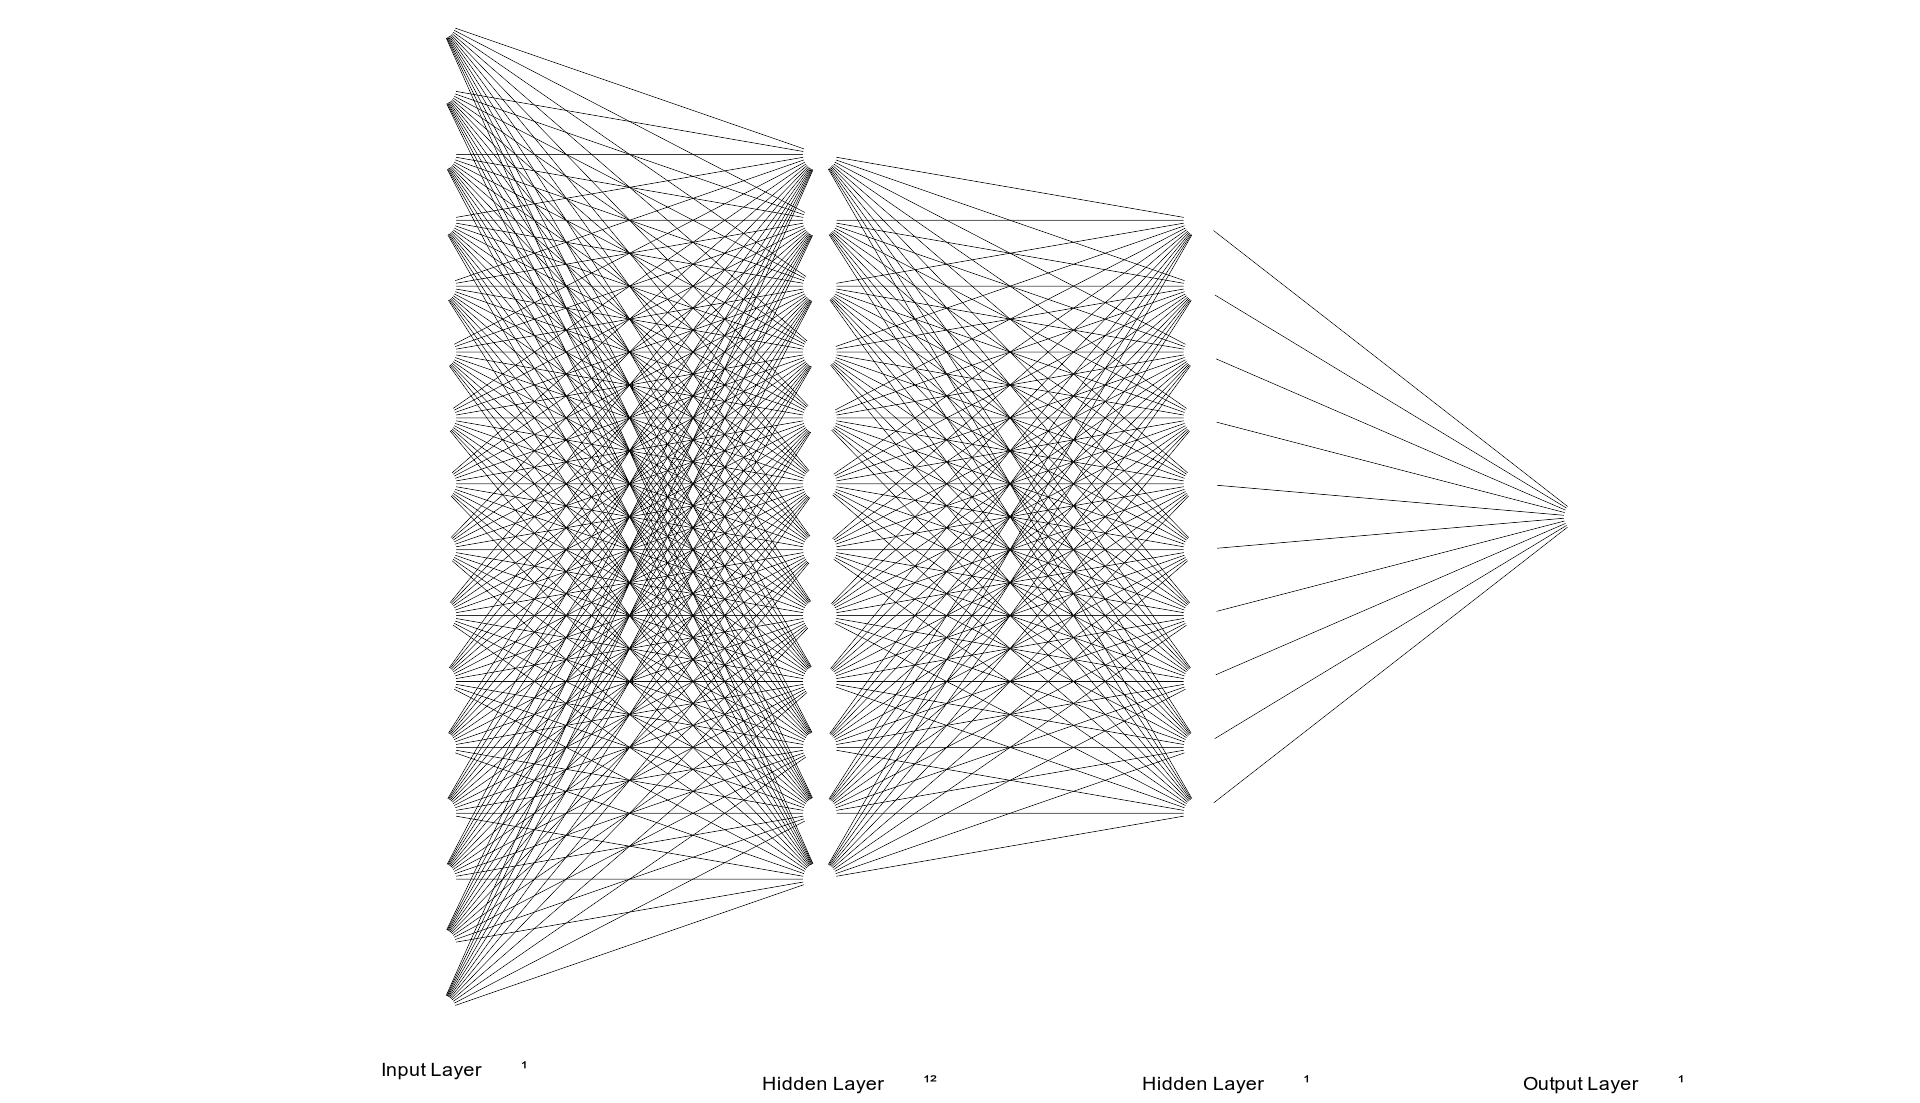
\includegraphics[keepaspectratio]{slides_files/figure-pdf/bfc06c80-466b-4ab4-b649-53f383e71ad1-1-../../assets/images/example.png}}

\textbf{Attribution}: LeNail, (2019). NN-SVG: Publication-Ready Neural
Network Architecture Schematics. Journal of Open Source Software, 4(33),
747, https://doi.org/10.21105/joss.00747
(\href{https://github.com/alexlenail/NN-SVG}{GitHub})

\section{Definnig AI}\label{definnig-ai}

\subsection{Survey}\label{survey}

Perceptions and Attitudes Toward Artificial Intelligence.

\begin{itemize}
\tightlist
\item
  The majority of students exhibit a generally positive disposition
  towards AI. If your perspective differs, please elaborate.
\item
  There is a wide range of opinions regarding the probability of
  catastrophic outcomes due to AI (P(doom)).
\item
  A relatively small number of students express concern about AI
  replacing their jobs.
\item
  Few students perceive current AI systems as genuinely intelligent.
\item
  Views on Artificial General Intelligence (AGI) and Super-intelligence
  vary significantly.
\item
  The primary concerns surrounding AI include potential job displacement
  and misuse, with privacy issues also noted.
\item
  Many students regard the medical and healthcare sectors as areas where
  AI could exert significant influence.
\item
  A substantial portion of students believes that AI is excessively
  hyped.
\item
  Fewer than 20\% of the students possess substantial experience in
  artificial intelligence.
\end{itemize}

\subsection{Why definning AI?}\label{why-definning-ai}

\begin{itemize}
\item
  \textbf{Enhancing Clarity and Communication:} Establishing a mutual
  understanding of evaluation criteria, benchmarking tests, and
  milestones.
\item
  \textbf{Addressing Ethical, Social, and Legal Implications:} Enabling
  policymakers to develop regulations that minimize AI-related risks.
\end{itemize}

\subsection{An operational definition}\label{an-operational-definition}

\begin{quote}
** (Wang 2019)**

To the larger community of computer science and information technology,
AI is usually identified by the techniques grown from it, which at
different periods may include \textbf{theorem proving},
\textbf{heuristic search}, \textbf{game playing}, \textbf{expert
systems}, \textbf{neural networks}, \textbf{Bayesian networks},
\textbf{data mining}, \textbf{agents}, and recently, \textbf{deep
learning}.
\end{quote}

\subsection{Context}\label{context}

\begin{itemize}
\tightlist
\item
  Significant \textbf{hype}.
\item
  Several leading companies, including
  \href{https://deepmind.google}{DeepMind} and
  \href{https://openai.com}{OpenAI}, are primarily focused on the
  development of \textbf{artificial general intelligence} (AGI).
\item
  Should AGI become a reality, \textbf{its implications could profoundly
  impact various aspects of our lives}, including education, employment,
  economic structures, and scientific advancements.
\end{itemize}

AI thus has great potential to influence the course of your lives. It is
therefore relevant to take the time to define what AI is and to explore
its different approaches.

I should warn you right away that there is no consensus on the
definition of AI, nor on the definition of intelligence.

\begin{center}\rule{0.5\linewidth}{0.5pt}\end{center}

\pandocbounded{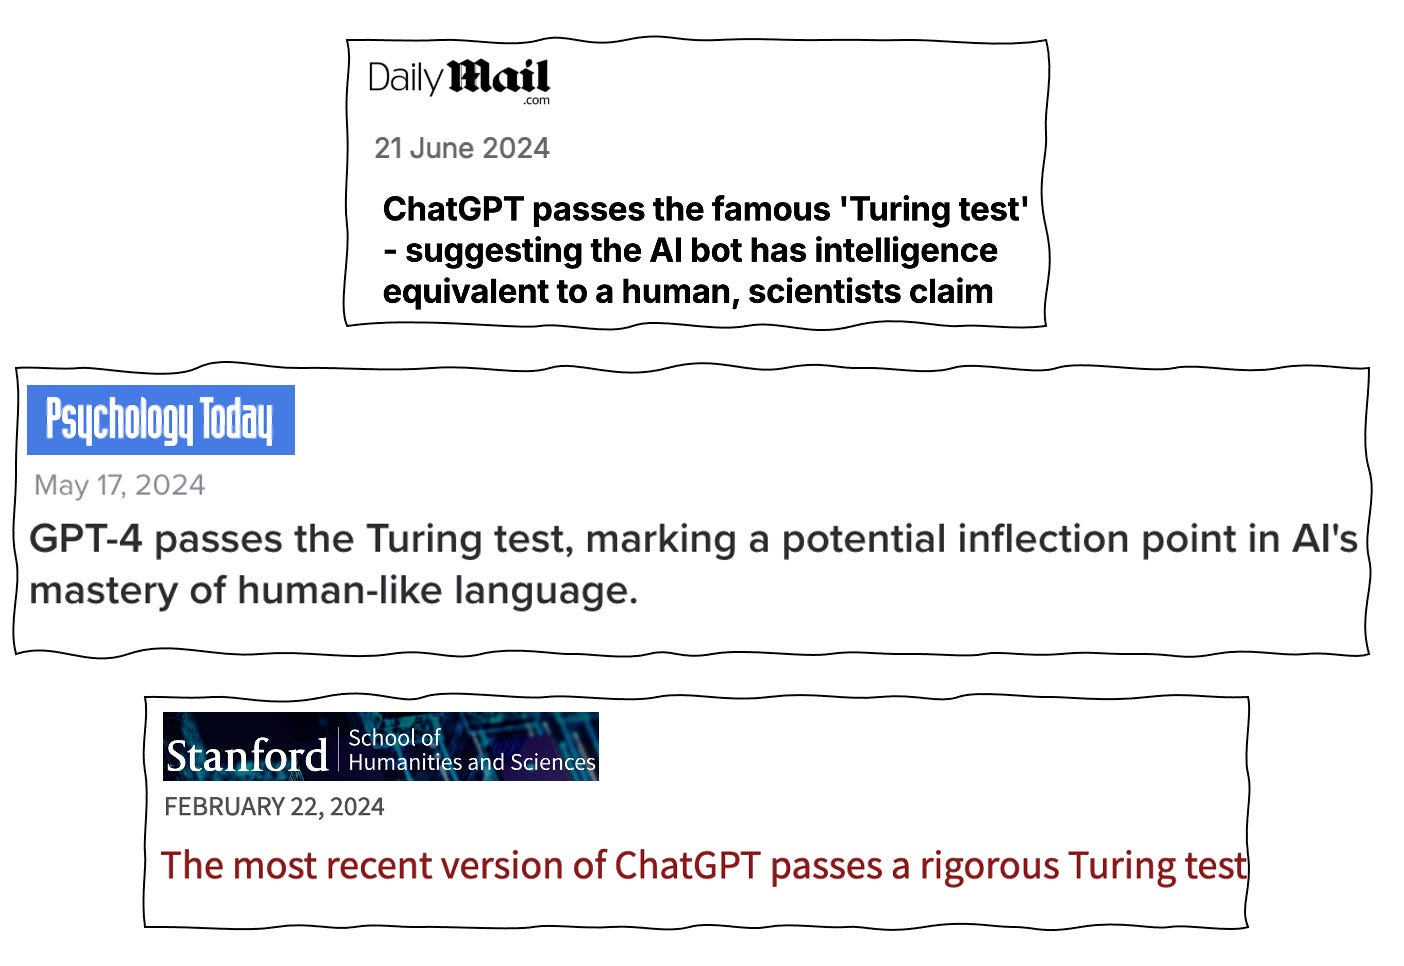
\includegraphics[keepaspectratio]{slides_files/mediabag/4fa37e16-8495-4038-8.jpg}}

\textbf{Attribution:} Melanie Mitchell, Substack post titled:
\href{https://aiguide.substack.com/p/the-turing-test-and-our-shifting}{The
Turing Test and Our Shifting Conceptions of Intelligence}, August 15,
2024.

\subsection{The complex nature of
intelligence}\label{the-complex-nature-of-intelligence}

. . .

\begin{itemize}
\item
  \textbf{``Artificial''} pertains to the creation of entities or
  phenomena that mimic natural processes using technology or synthetic
  materials, a definition broadly recognized and accepted.
\item
  Therefore, defining \textbf{``artificial intelligence''} fundamentally
  requires us to first clarify what we mean by
  \textbf{``intelligence.''} Surprisingly, ``{[}d{]}espite a long
  history of research and debate, there is still no standard definition
  of intelligence.'' (Legg and Hutter 2007)
\end{itemize}

\subsection{How do you define
intelligence?}\label{how-do-you-define-intelligence}

\begin{itemize}
\tightlist
\item
  What are the \textbf{characteristics} you associate with
  \textbf{intelligence}?
\end{itemize}

\subsection{Essential abilities}\label{essential-abilities}

\begin{quote}
**
\href{https://cogs.indiana.edu/directory/faculty/profile.php?faculty=dughof}{Douglas
Hofstadter}**

No one knows where the borderline between non-intelligent behavior and
intelligent behavior lies, in fact, to suggest that a sharp border
exists is probably silly. But essential abilities for intelligence are
certainly:

\begin{enumerate}
\def\labelenumi{\arabic{enumi}.}
\tightlist
\item
  to respond to situations very \textbf{flexibly};
\item
  to take advantage of \textbf{fortuitous} circumstances;
\item
  to make sense out of \textbf{ambiguous} or \textbf{contradictory
  messages};
\item
  to recognise the \textbf{relative importance of different elements} of
  a situation;
\item
  to find \textbf{similarities} between situations despite differences
  which may separate them;
\item
  to draw \textbf{distinctions} between situations despite similarities
  which may link them;
\item
  to \textbf{synthesize} new concepts by taking old concepts and putting
  them together in new ways;
\item
  to come up with \textbf{ideas which are novel.}''
\end{enumerate}
\end{quote}

For certain complex concepts, drawing a clear boundary can prove
challenging. Take the concept of life, for example. Humans, plants, and
insects are considered living, as are microorganisms such as bacteria.
However, viruses and viroids are not.

\subsection{\texorpdfstring{\href{https://fchollet.com}{François
Chollet}, Creator of
\href{https://keras.io}{Keras}}{François Chollet, Creator of Keras}}\label{franuxe7ois-chollet-creator-of-keras}

\begin{quote}
** François Chollet**

Real intelligence is not about mastering an individual skill, he argued,
but about \textbf{taking what has been learned and applying it to a new,
different situation}.

In his view, intelligence is the ability to \textbf{efficiently acquire
new skills} that training did not prepare for, with the goal of
accomplishing tasks that are sufficiently different from those a system
has seen before.

\textbf{The wider the scope of the new skills, the closer the computer
comes to achieving artificial general intelligence.}

``If you can make the learning process as information-efficient as a
human mind, then you've got AGI,'' Chollet said.

So far, machines lag far behind, approximately 10,000 times less
efficient than human brains. For instance, \textbf{it took millions of
images to teach computers to recognize pictures of cats, whereas humans
learn to identify them based on only one or two examples}.

Savage (2024)
\end{quote}

\subsection{Thinking, acting, humanly,
rationally}\label{thinking-acting-humanly-rationally}

Russell \& Norvig considers two axes: thinking vs behaviour, human vs
rationality.

\begin{longtable}[]{@{}
  >{\raggedright\arraybackslash}p{(\linewidth - 4\tabcolsep) * \real{0.1757}}
  >{\raggedright\arraybackslash}p{(\linewidth - 4\tabcolsep) * \real{0.4189}}
  >{\raggedright\arraybackslash}p{(\linewidth - 4\tabcolsep) * \real{0.4054}}@{}}
\toprule\noalign{}
\begin{minipage}[b]{\linewidth}\raggedright
\end{minipage} & \begin{minipage}[b]{\linewidth}\raggedright
Thinking
\end{minipage} & \begin{minipage}[b]{\linewidth}\raggedright
Acting
\end{minipage} \\
\midrule\noalign{}
\endhead
\bottomrule\noalign{}
\endlastfoot
Human-like & thinking humanly (simulation) & acting humanly (Turing
test) \\
Rationality & thinking rationally (logic) & acting rationally (agent) \\
\end{longtable}

\textbf{See also} the appendix -- Section~9 On Defining Artificial
Intelligence

The question of intelligence has been the subject of much debate in the
literature and the media, particularly when it comes to animals or
computers. This abundance of information can bias our thinking.

A simple thought experiment might offer a new perspective: would you be
able to recognize intelligence in an extraterrestrial entity?

\subsection{Rationality}\label{rationality}

\pandocbounded{\includegraphics[keepaspectratio]{slides_files/mediabag/Spock_and_T-Pring.jpg}}

\begin{quote}
** (Mohammed, Sookram, and Saridakis 2019)**

Rationality involves the \textbf{evaluation of choices to achieve a goal
or to find the optimal solution to a problem}. Simon (1972, p.~161)
defined rationality as ``a style of behavior that is appropriate to the
\textbf{achievement of given goals}, within the \textbf{limits imposed
by given conditions and constraints}.''
\end{quote}

\textbf{Attribution:}
\href{https://commons.wikimedia.org/wiki/File:Spock_and_T\%27Pring.jpg}{NBC
Television, Public domain, via Wikimedia Commons}

\section{Narrow vs General AI}\label{narrow-vs-general-ai}

\subsection{Artificial General Intelligence
(AGI)}\label{artificial-general-intelligence-agi}

Artificial general intelligence (AGI) refers to a form of artificial
intelligence (AI) that either \textbf{equals} or \textbf{exceeds human
proficiency} across a \textbf{diverse array of cognitive functions}.

AKA \textbf{human-level intelligence}. As opposed to \textbf{narrow
intelligence}, the current status of AI, which is designed to perform a
specific task or a limited range of tasks, operating under predefined
constraints and without general cognitive abilities.

\subsection{AlphaFold (1, 2, \& 3)}\label{alphafold-1-2-3}

I repeat, \textbf{there is nothing wrong with narrow AI}.

\begin{itemize}
\item
  «Two papers in this week's issue dramatically expand our structural
  understanding of proteins. Researchers at \textbf{DeepMind}, Google's
  London-based sister company, present the latest version of their
  \textbf{AlphaFold} neural network.»

  \begin{itemize}
  \tightlist
  \item
    Jumper et al.~(2021)
  \end{itemize}
\end{itemize}

\subsection{AI effect/paradox}\label{ai-effectparadox}

\begin{quote}
** (Wang 2019)**

(\(\ldots\)) as soon as a computer system is built to solve a problem
successfully, the problem is no longer ``only solvable by the human
mind,'' so does not need intelligence anymore. Consequently,
``\textbf{AI is whatever hasn't been done yet}'' (Hofstadter, 1979;
Schank, 1991), which is known as ``\textbf{the AI Effect}'' (McCorduck
2004).
\end{quote}

The paradox of AI is quite fascinating. In the early days of AI,
researchers focused on problems like differential equations or chess.

Each time a computer solves one of these major problems, we come to
think that perhaps that problem didn't really require intelligence to be
solved after all.

The defeat of Garry Kasparov at the hands of IBM's Watson is a perfect
example.

\section{Impact}\label{impact}

\subsection{Economical}\label{economical}

\begin{quote}
**
\href{https://www.mckinsey.com/industries/technology-media-and-telecommunications/our-insights/beyond-the-hype-capturing-the-potential-of-ai-and-gen-ai-in-tmt\#/}{Beyond
the hype: Capturing the potential of AI and gen AI in tech, media, and
telecom} 2024-02-22**

McKinsey research estimates that \textbf{gen AI} could add to the
economy between \textbf{\$2.6 trillion and \$4.4 trillion annually}
while increasing the impact of all artificial intelligence by 15 to 40
percent.

In fact, it seems possible that \textbf{within the next three years},
\textbf{anything not connected to AI will be considered obsolete or
ineffective}.
\end{quote}

\subsection{Subfields of AI}\label{subfields-of-ai}

\begin{enumerate}
\def\labelenumi{\arabic{enumi}.}
\tightlist
\item
  \textbf{Machine Learning:} Credit card fraud detection
\item
  \textbf{Deep Learning:} Image and facial recognition
\item
  \textbf{Natural Language Processing:} Virtual assistants like Siri or
  Alexa
\item
  \textbf{Computer Vision:} Autonomous vehicles
\item
  \textbf{Robotics:} Industrial automation in manufacturing
\item
  \textbf{Expert Systems:} Medical diagnosis support
\item
  \textbf{Speech Recognition:} Voice-to-text transcription services
\item
  \textbf{Planning and Decision Making:} Supply chain optimization
\item
  \textbf{Reinforcement Learning:} Game AI in complex strategy games
\item
  \textbf{Knowledge Representation:} Semantic web technologies for
  information retrieval
\end{enumerate}

\subsection{Our Final Invention}\label{our-final-invention}

\begin{quote}
** (Russell and Norvig 2020)**

\textbf{AI} expert Kai-Fu Lee predicts that its \textbf{impact} will be
\textbf{``more than anything in the history of mankind.''}
\end{quote}

\begin{center}\rule{0.5\linewidth}{0.5pt}\end{center}

\url{https://youtu.be/ixgunKpy61s}

\href{https://youtu.be/ixgunKpy61s}{What Does the AI Boom Really Mean
for Humanity? \textbar{} The Future With Hannah Fry}. Bloomberg
Originals, posted on YouTube on 2024-09-12.

\begin{center}\rule{0.5\linewidth}{0.5pt}\end{center}

\url{https://youtu.be/sK5_pQV_QEA}

\subsection{Questions}\label{questions}

\begin{itemize}
\item
  Can the concept of intelligence be considered \textbf{independently}
  of the entities that express it? This is the problem of
  \textbf{embodiment}.
\item
  Can a \textbf{machine} exhibit human-level intelligence?
\item
  Is it possible to \textbf{dissociate} the following concepts from that
  of intelligence?

  \begin{itemize}
  \tightlist
  \item
    \textbf{Agency}.
  \item
    \textbf{Sentience}.
  \item
    \textbf{Consciousness}.
  \item
    \textbf{Emotions}.
  \item
    \textbf{Language}.
  \item
    \textbf{Mind}.
  \end{itemize}
\item
  Can an AI \textbf{suffer}?
\end{itemize}

For me, an interesting definition of intelligence would be similar in
nature to that of computation.

Using \textbf{computation} as an analogous concept can help clarify this
question. Theoretically, computation is often considered in an abstract
manner, independent of any physical implementation. The
\textbf{Church-Turing theorem}, a fundamental principle in computer
science, states that any computation that can be performed by a machine
(specifically, a Turing machine) is universally applicable. This implies
that the concept of computation can exist independently of its hardware
or specific physical form.

I must confess: until 2022, I was rather skeptical. I often drew a
parallel between artificial intelligence and alchemy. Alchemists never
succeeded in transmuting lead into gold because it is a physical
process, but their approach led to the development of chemistry.
Similarly, we may never be able to replicate human intelligence, but the
impacts of AI are immense and often unexpected, like the garbage
collector introduced by Lisp.

Then, it struck me: I am a scientist, and I wondered what it would mean
if we were not able to produce intelligence comparable to that of
humans.

Richard Feynman, who received the Nobel Prize in Physics in 1965,
famously said, ``What I cannot build. I do not understand.''

Why seek to dissociate intelligence from other concepts such as agency,
consciousness, and emotions? A computer system devoid of these
attributes seems, indeed, far less daunting.

\subsection{Deepen the Reflection}\label{deepen-the-reflection}

\pandocbounded{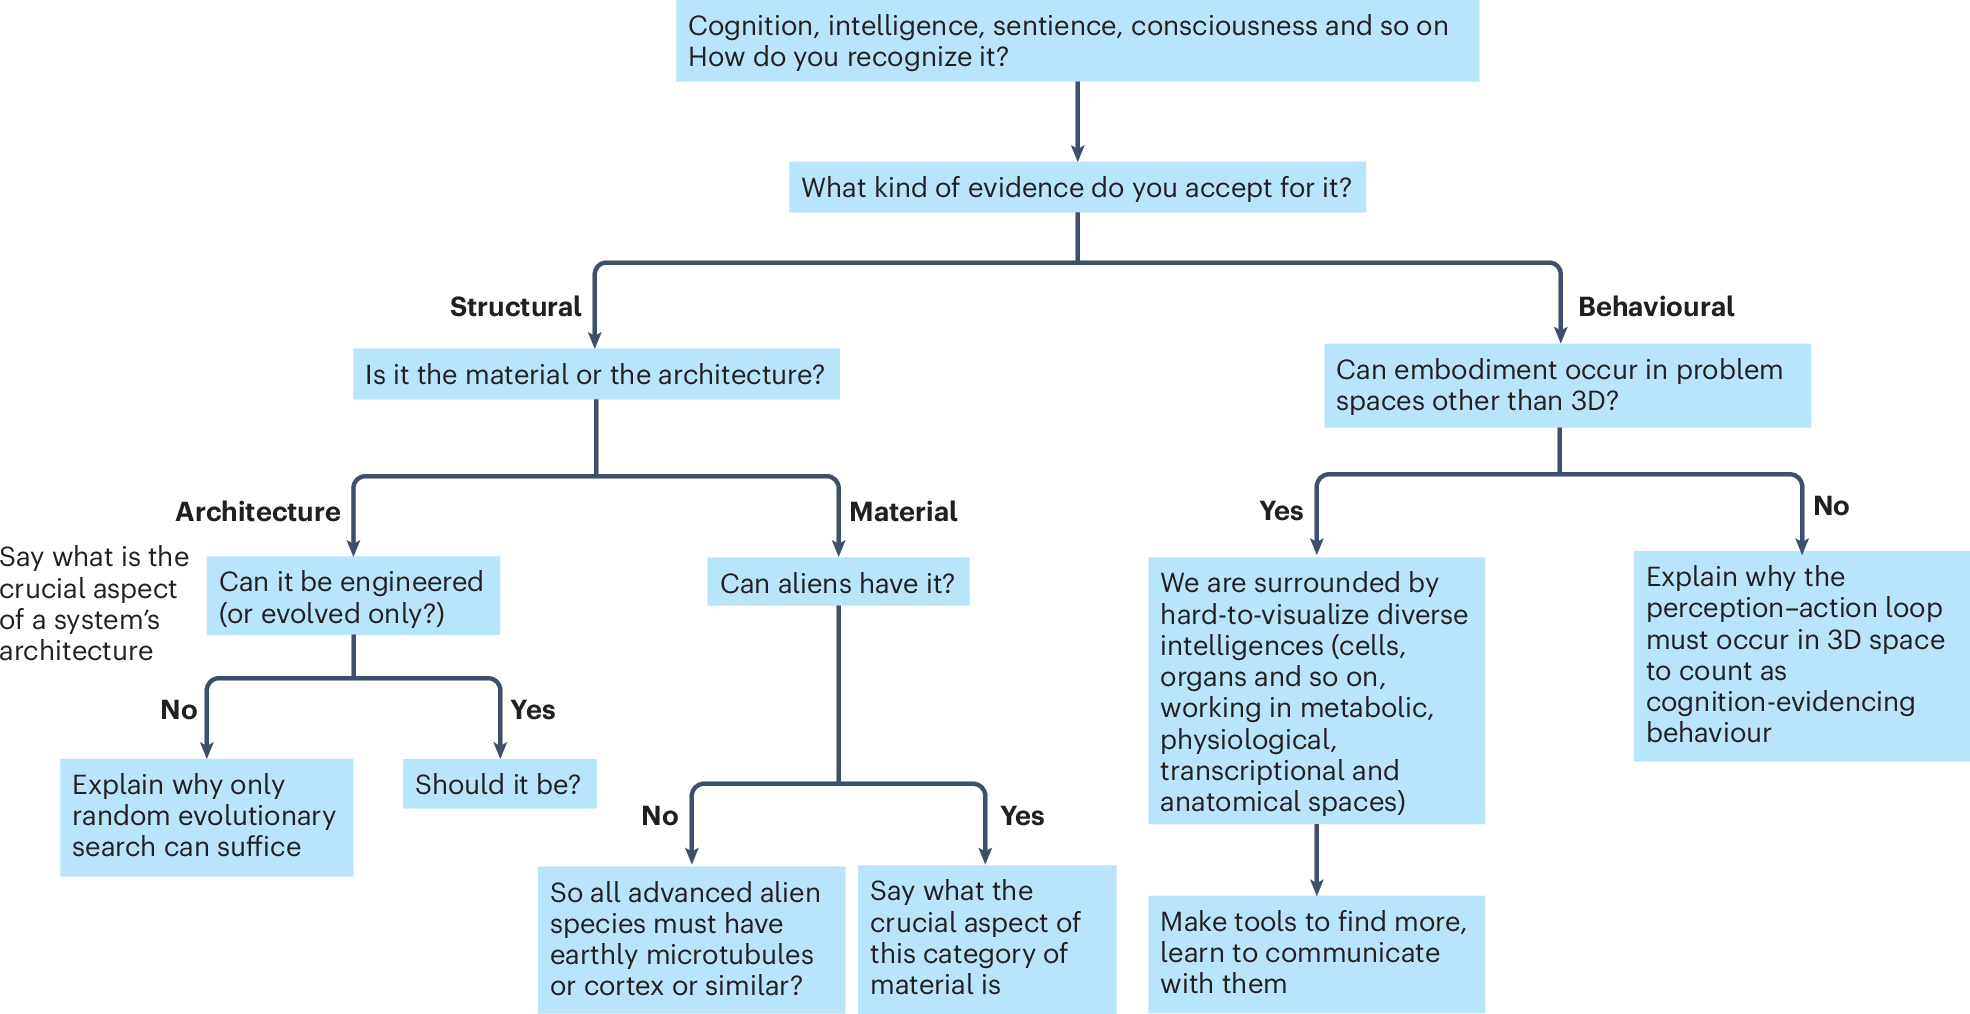
\includegraphics[keepaspectratio]{slides_files/mediabag/42256_2024_955_Fig1_.png}}

Rouleau, N. \& Levin, M. (2024).
\href{(https://doi.org/10.1038/s42256-024-00955-y)}{Discussions of
machine versus living intelligence need more clarity.} \emph{Nature
Machine Intelligence}, 6(12), 1424--1426.

\section{Prologue}\label{prologue}

\subsection{Summary}\label{summary}

\begin{itemize}
\tightlist
\item
  \textbf{Discussed} the syllabus
\item
  \textbf{Distinguish} the concept of artificial intelligence from the
  concept of machine learning
\item
  \textbf{Distinguish} symbolic AI from connectionnist AI
\item
  \textbf{Explored} the various definitions of ``artificial
  intelligence''
\end{itemize}

\subsection{Next lecture}\label{next-lecture}

\begin{itemize}
\tightlist
\item
  Introduction to machine learning
\end{itemize}

\subsection{References}\label{references}

Bennett, Max S. 2023. \emph{A Brief History of Intelligence: Evolution,
AI, and the Five Breakthroughs That Made Our Brains}. First edition. New
York: Mariner Books.

Jumper, John, Richard Evans, Alexander Pritzel, Tim Green, Michael
Figurnov, Olaf Ronneberger, Kathryn Tunyasuvunakool, et al.~2021.
``{Highly accurate protein structure prediction with AlphaFold}.''
\emph{Nature}, 1--11. \url{https://doi.org/10.1038/s41586-021-03819-2}.

Legg, Shane, and Marcus Hutter. 2007. ``{A Collection of Definitions of
Intelligence}.'' In \emph{Advances in Artificial General Intelligence:
Concepts, Architectures and Algorithms:}, 17--24. NLD: IOS Press.
\url{https://doi.org/10.5555/1565455.1565458}.

McCorduck, Pamela. 2004. \emph{{Machines Who Think, A Personal Inquiry
into the History and Prospects of Artificial Intelligence}}. Taylor \&
Francis Group, LLC. \url{https://doi.org/10.1201/9780429258985}.

Mohammed, Anne-Marie, Sandra Sookram, and George Saridakis. 2019.
``Rationality.'' In \emph{Encyclopedia of Law and Economics}, edited by
Alain Marciano and Giovanni Battista Ramello, 1766--74. New York, NY:
Springer New York. \url{https://doi.org/10.1007/978-1-4614-7753-2_404}.

Newell, Allen, and Herbert A. Simon. 1976. ``Computer Science as
Empirical Inquiry: Symbols and Search.'' \emph{Commun. ACM} 19 (3):
113--26. \url{https://doi.org/10.1145/360018.360022}.

Nilsson, Nils J. 2005. ``Human-Level Artificial Intelligence? Be
Serious!'' \emph{AI Mag.} 26 (4): 68--75.
\url{https://doi.org/10.1609/AIMAG.V26I4.1850}.

Poole, David L., and Alan K. Mackworth. 2023. \emph{Artificial
Intelligence: Foundations of Computational Agents}. 3rd ed.~Cambridge
University Press.

Russell, Stuart, and Peter Norvig. 2020. \emph{Artificial Intelligence:
A Modern Approach}. 4th ed.~Pearson. \url{http://aima.cs.berkeley.edu/}.

Savage, Neil. 2024. ``Beyond Turing: Testing LLMs for Intelligence.''
\emph{Commun. ACM}, June. \url{https://doi.org/10.1145/3673427}.

Strickland, Eliza. 2021. ``The Turbulent Past and Uncertain Future of
AI: Is There a Way Out of AI's Boom-and-Bust Cycle?'' \emph{IEEE
Spectrum} 58 (10): 26--31.
\url{https://doi.org/10.1109/MSPEC.2021.9563956}.

Wang, Pei. 2019. ``On Defining Artificial Intelligence.'' \emph{Journal
of Artificial General Intelligence} 10 (2): 1--37.
\url{https://doi.org/10.2478/jagi-2019-0002}.

\section{Appendix: On Defining Artificial
Intelligence}\label{appendix-on-defining-artificial-intelligence}

\subsection{Wang (2019)}\label{wang-2019}

An \textbf{agent} and its \textbf{interaction with the environment} are
specified as a tuple: \[
\langle P,S,A \rangle
\] where

\begin{itemize}
\tightlist
\item
  \(P\) represents a sequence of \textbf{input signals},
  \(P = \langle p_0,\ldots,p_t \rangle\)
\item
  \(S\) represents a sequence of \textbf{internal states},
  \(S = \langle s_0,\ldots,s_t \rangle\)
\item
  \(A\) represents a sequence of \textbf{actions},
  \(A = \langle a_0,\ldots,a_t \rangle\)
\end{itemize}

For a sequence of moments, \(0,\ldots,t\).

\subsection{Human (H) vs Computer (C)}\label{human-h-vs-computer-c}

\begin{quote}
** (Wang 2019)**

AI is conceived as computer systems that are similar to the human mind
in a certain sense, though a computer and a human mind cannot be
identical in all aspects.
\end{quote}

\[
\langle P^H,S^H,A^H \rangle \approx \langle P^C,S^C,A^C \rangle
\]

. . .

Wang (2019) proposes 5 perspectives: \textbf{Structure-AI},
\textbf{Behavior-AI}, \textbf{Capability-AI}, \textbf{Function-AI}, and
\textbf{Principle-AI}.

\subsection{1. Structure-AI}\label{structure-ai}

(brain modelling, cognitive science)

\begin{quote}
** (Wang 2019)**

I call this type of definition \textbf{``Structure-AI,''} since it
requires an AI system to go through \textbf{isomorphic states} or
structure changes as the brain does when they are given \textbf{similar
input}, which will produce \textbf{similar output}, so the three
components of the two are pairwise similar to each other:
\end{quote}

\[
 P^H \approx P^C, S^H \approx S^C, A^H \approx A^C 
\]

\subsection{2. Behaviour-AI}\label{behaviour-ai}

(Turing Test)

\begin{quote}
** (Wang 2019)**

One way to acknowledge a human-like mind without demanding a human-like
brain is to associate intelligence to the external behaviors of the
agent. After all, \textbf{if an agent behaves like a human, it should be
considered as intelligent}, no matter whether it looks like a human,
either inside or outside.
\end{quote}

\[
 P^H \approx P^C, A^H \approx A^C 
\]

\subsection{3. Capability-AI (Employment
Test)}\label{capability-ai-employment-test}

\begin{quote}
** (Wang 2019)**

In the agent framework, it means that \(C\) is similar to \(H\) in the
sense that there are moments \(i\) and \(j\) that:
\end{quote}

\[
 p_i^C \approx p_j^H, a_i^C \approx a_j^H 
\]

\begin{quote}
** (Wang 2019)**

the action (solution) the computer produces for a percept (problem) is
similar to the action produced by a human to a similar percept
(\(\ldots\)) In this way, \textbf{the intelligence of a system is
identified by a set of problems it can solve}, while whether they are
solved in the ``human way'' does not matter.
\end{quote}

\subsection{Capability-AI (contd)}\label{capability-ai-contd}

\begin{quote}
** (Nilsson 2005)**

``I suggest we replace the Turing test by something I will call the
`employment test.' To pass the employment test, \textbf{AI programs must
be able to perform the jobs ordinarily performed by humans}. Progress
toward human-level AI could then be measured by the fraction of these
jobs that can be acceptably performed by machines''
\end{quote}

\subsection{4. Function-AI}\label{function-ai}

\begin{quote}
** (Wang 2019)**

In the agent framework, this \textbf{``Function-AI''} perspective takes
\(C\) to be similar to \(H\) in the sense that there are moments \(i\)
and \(j\) that:
\end{quote}

\[
 a_i^C \approx f^C(p_i^C), a_j^H \approx f^H(p_j^H), f^C \approx f^H
\]

\begin{quote}
** (Wang 2019)**

Here the function can correspond to searching, \textbf{reasoning},
\textbf{learning}, etc., and since \textbf{the focus is on the
functions} (i.e., input-output mappings), the concrete input and output
values of the two agents do not have to be similar to each other.
\end{quote}

\subsection{6. Principle-AI (rationality,
logicist)}\label{principle-ai-rationality-logicist}

\begin{quote}
** (Wang 2019)**

As in any field, there are researchers in AI trying to find
\textbf{fundamental principles} that can uniformly explain the relevant
phenomena. Here the idea comes from the usage of intelligence as a form
of \emph{rationality} (\(\ldots\)) that can make the
\textbf{best-possible decision} in various situations, according to the
experience or history of the system.
\end{quote}

\[
 A^C = F^C(P^C), A^H = F^H(P^H), F^C \approx F^H
\]

\begin{quote}
** (Wang 2019)**

The above \(F\) is often not formally specified, but described
informally as a certain \textbf{``principle,''} which is not merely
about a single type of problem and its solution, but about \textbf{the
agent's life-long history in various situations}, when dealing with
various types of problems.
\end{quote}

\subsection{Code of the day}\label{code-of-the-day}

\begin{Shaded}
\begin{Highlighting}[]
\CommentTok{\#!/usr/bin/env python3}
\CommentTok{\# {-}*{-} Mode: Python {-}*{-}}
\CommentTok{\# ai\_lecture{-}01.py}
\CommentTok{\# Author          : Marcel Turcotte \& ChatGPT 5}
\CommentTok{\# Created On      : Tue Feb 13 16:29:41 2024}
\CommentTok{\# Last Modified By: Marcel Turcotte}
\CommentTok{\# Last Modified On: Thu Aug 28 15:03:14 EDT 2025}

\CommentTok{\# In 2024, I developed the initial version of this script. }
\CommentTok{\# This year, I used ChatGPT to revise the code to align with the most recent API version, }
\CommentTok{\# enhance its educational value by incorporating detailed comments, }
\CommentTok{\# and improve its suitability as an instructive example.}

\CommentTok{"""}
\CommentTok{Didactic example: translate EN{-}\textgreater{}Canadian French, then synthesize audio in EN \& FR.}

\CommentTok{CLI options:}
\CommentTok{    {-}{-}format : audio output format (mp3, wav, etc.)}
\CommentTok{    {-}{-}voice  : TTS voice (e.g., nova, alloy, verse, etc.)}
\CommentTok{    {-}{-}model  : TTS model (tts{-}1{-}hd for high quality, gpt{-}4o{-}mini{-}tts for low latency)}

\CommentTok{Examples:}
\CommentTok{    python ai\_lecture{-}01.py {-}{-}format mp3 {-}{-}voice nova {-}{-}model tts{-}1{-}hd}
\CommentTok{    python ai\_lecture{-}01.py {-}{-}format wav {-}{-}voice alloy {-}{-}model gpt{-}4o{-}mini{-}tts}
\CommentTok{"""}

\ImportTok{from}\NormalTok{ \_\_future\_\_ }\ImportTok{import}\NormalTok{ annotations}

\ImportTok{import}\NormalTok{ os}
\ImportTok{import}\NormalTok{ argparse}
\ImportTok{from}\NormalTok{ pathlib }\ImportTok{import}\NormalTok{ Path}

\ImportTok{from}\NormalTok{ openai }\ImportTok{import}\NormalTok{ OpenAI, APIError, APIConnectionError, APITimeoutError}

\CommentTok{\# {-}{-}{-}{-}{-}{-}{-}{-}{-}{-}{-}{-}{-}{-}{-}{-}{-}{-}{-}{-}{-}{-}{-}{-}{-}{-}{-}{-}{-}{-}{-}{-}{-}{-}{-}{-}{-}{-}{-}{-}{-}{-}{-}{-}{-}{-}{-}{-}{-}{-}{-}{-}{-}{-}{-}}
\CommentTok{\# Configuration}
\CommentTok{\# {-}{-}{-}{-}{-}{-}{-}{-}{-}{-}{-}{-}{-}{-}{-}{-}{-}{-}{-}{-}{-}{-}{-}{-}{-}{-}{-}{-}{-}{-}{-}{-}{-}{-}{-}{-}{-}{-}{-}{-}{-}{-}{-}{-}{-}{-}{-}{-}{-}{-}{-}{-}{-}{-}{-}}

\NormalTok{client }\OperatorTok{=}\NormalTok{ OpenAI()  }\CommentTok{\# Reads OPENAI\_API\_KEY from environment}

\CommentTok{\# {-}{-}{-}{-}{-}{-}{-}{-}{-}{-}{-}{-}{-}{-}{-}{-}{-}{-}{-}{-}{-}{-}{-}{-}{-}{-}{-}{-}{-}{-}{-}{-}{-}{-}{-}{-}{-}{-}{-}{-}{-}{-}{-}{-}{-}{-}{-}{-}{-}{-}{-}{-}{-}{-}{-}}
\CommentTok{\# Text Utilities}
\CommentTok{\# {-}{-}{-}{-}{-}{-}{-}{-}{-}{-}{-}{-}{-}{-}{-}{-}{-}{-}{-}{-}{-}{-}{-}{-}{-}{-}{-}{-}{-}{-}{-}{-}{-}{-}{-}{-}{-}{-}{-}{-}{-}{-}{-}{-}{-}{-}{-}{-}{-}{-}{-}{-}{-}{-}{-}}

\KeywordTok{def}\NormalTok{ translate\_to\_canadian\_french(input\_text: }\BuiltInTok{str}\NormalTok{) }\OperatorTok{{-}\textgreater{}} \BuiltInTok{str}\NormalTok{:}
    \CommentTok{"""Translate English text to Canadian French (CSI4106→CSI4506)."""}
\NormalTok{    instructions }\OperatorTok{=}\NormalTok{ (}
        \StringTok{"You are a careful translator. Translate the user\textquotesingle{}s English text into Canadian French. "}
        \StringTok{"Preserve technical terms and course names. "}
        \StringTok{\textquotesingle{}If the course code "CSI4106" appears, translate it as "CSI4506".\textquotesingle{}}
\NormalTok{    )}

    \ControlFlowTok{try}\NormalTok{:}
\NormalTok{        resp }\OperatorTok{=}\NormalTok{ client.responses.create(}
\NormalTok{            model}\OperatorTok{=}\StringTok{"gpt{-}4o"}\NormalTok{,}
\NormalTok{            instructions}\OperatorTok{=}\NormalTok{instructions,}
            \BuiltInTok{input}\OperatorTok{=}\NormalTok{input\_text,}
\NormalTok{            temperature}\OperatorTok{=}\FloatTok{0.2}\NormalTok{,}
\NormalTok{            max\_output\_tokens}\OperatorTok{=}\DecValTok{1200}\NormalTok{,}
\NormalTok{        )}
        \ControlFlowTok{return}\NormalTok{ resp.output\_text }\KeywordTok{or} \StringTok{""}
    \ControlFlowTok{except}\NormalTok{ (APIConnectionError, APITimeoutError) }\ImportTok{as}\NormalTok{ net\_err:}
        \BuiltInTok{print}\NormalTok{(}\SpecialStringTok{f"[Network issue] }\SpecialCharTok{\{}\NormalTok{net\_err}\SpecialCharTok{\}}\SpecialStringTok{"}\NormalTok{)}
    \ControlFlowTok{except}\NormalTok{ APIError }\ImportTok{as}\NormalTok{ api\_err:}
        \BuiltInTok{print}\NormalTok{(}\SpecialStringTok{f"[OpenAI API error] }\SpecialCharTok{\{}\NormalTok{api\_err}\SpecialCharTok{\}}\SpecialStringTok{"}\NormalTok{)}
    \ControlFlowTok{except} \PreprocessorTok{Exception} \ImportTok{as}\NormalTok{ e:}
        \BuiltInTok{print}\NormalTok{(}\SpecialStringTok{f"[Unexpected error] }\SpecialCharTok{\{}\NormalTok{e}\SpecialCharTok{\}}\SpecialStringTok{"}\NormalTok{)}
    \ControlFlowTok{return} \StringTok{""}

\CommentTok{\# {-}{-}{-}{-}{-}{-}{-}{-}{-}{-}{-}{-}{-}{-}{-}{-}{-}{-}{-}{-}{-}{-}{-}{-}{-}{-}{-}{-}{-}{-}{-}{-}{-}{-}{-}{-}{-}{-}{-}{-}{-}{-}{-}{-}{-}{-}{-}{-}{-}{-}{-}{-}{-}{-}{-}}
\CommentTok{\# Audio Utilities}
\CommentTok{\# {-}{-}{-}{-}{-}{-}{-}{-}{-}{-}{-}{-}{-}{-}{-}{-}{-}{-}{-}{-}{-}{-}{-}{-}{-}{-}{-}{-}{-}{-}{-}{-}{-}{-}{-}{-}{-}{-}{-}{-}{-}{-}{-}{-}{-}{-}{-}{-}{-}{-}{-}{-}{-}{-}{-}}

\KeywordTok{def}\NormalTok{ synthesize\_speech(}
\NormalTok{    text: }\BuiltInTok{str}\NormalTok{,}
\NormalTok{    output\_path: Path,}
    \OperatorTok{*}\NormalTok{,}
\NormalTok{    model: }\BuiltInTok{str} \OperatorTok{=} \StringTok{"tts{-}1{-}hd"}\NormalTok{,}
\NormalTok{    voice: }\BuiltInTok{str} \OperatorTok{=} \StringTok{"nova"}\NormalTok{,}
\NormalTok{    response\_format: }\BuiltInTok{str} \OperatorTok{=} \StringTok{"mp3"}\NormalTok{,}
\NormalTok{) }\OperatorTok{{-}\textgreater{}} \BuiltInTok{bool}\NormalTok{:}
    \CommentTok{"""}
\CommentTok{    Stream synthesized speech to a file on disk.}
\CommentTok{    Returns True on success, False otherwise.}
\CommentTok{    """}
\NormalTok{    output\_path.parent.mkdir(parents}\OperatorTok{=}\VariableTok{True}\NormalTok{, exist\_ok}\OperatorTok{=}\VariableTok{True}\NormalTok{)}

    \ControlFlowTok{try}\NormalTok{:}
        \ControlFlowTok{with}\NormalTok{ client.audio.speech.with\_streaming\_response.create(}
\NormalTok{            model}\OperatorTok{=}\NormalTok{model,}
\NormalTok{            voice}\OperatorTok{=}\NormalTok{voice,}
            \BuiltInTok{input}\OperatorTok{=}\NormalTok{text,}
\NormalTok{            response\_format}\OperatorTok{=}\NormalTok{response\_format,}
\NormalTok{        ) }\ImportTok{as}\NormalTok{ response:}
\NormalTok{            response.stream\_to\_file(}\BuiltInTok{str}\NormalTok{(output\_path))}
        \ControlFlowTok{return} \VariableTok{True}
    \ControlFlowTok{except}\NormalTok{ (APIConnectionError, APITimeoutError) }\ImportTok{as}\NormalTok{ net\_err:}
        \BuiltInTok{print}\NormalTok{(}\SpecialStringTok{f"[Network issue] }\SpecialCharTok{\{}\NormalTok{net\_err}\SpecialCharTok{\}}\SpecialStringTok{"}\NormalTok{)}
    \ControlFlowTok{except}\NormalTok{ APIError }\ImportTok{as}\NormalTok{ api\_err:}
        \BuiltInTok{print}\NormalTok{(}\SpecialStringTok{f"[OpenAI API error] }\SpecialCharTok{\{}\NormalTok{api\_err}\SpecialCharTok{\}}\SpecialStringTok{"}\NormalTok{)}
    \ControlFlowTok{except} \PreprocessorTok{Exception} \ImportTok{as}\NormalTok{ e:}
        \BuiltInTok{print}\NormalTok{(}\SpecialStringTok{f"[Unexpected error] }\SpecialCharTok{\{}\NormalTok{e}\SpecialCharTok{\}}\SpecialStringTok{"}\NormalTok{)}
    \ControlFlowTok{return} \VariableTok{False}

\CommentTok{\# {-}{-}{-}{-}{-}{-}{-}{-}{-}{-}{-}{-}{-}{-}{-}{-}{-}{-}{-}{-}{-}{-}{-}{-}{-}{-}{-}{-}{-}{-}{-}{-}{-}{-}{-}{-}{-}{-}{-}{-}{-}{-}{-}{-}{-}{-}{-}{-}{-}{-}{-}{-}{-}{-}{-}}
\CommentTok{\# Example script logic}
\CommentTok{\# {-}{-}{-}{-}{-}{-}{-}{-}{-}{-}{-}{-}{-}{-}{-}{-}{-}{-}{-}{-}{-}{-}{-}{-}{-}{-}{-}{-}{-}{-}{-}{-}{-}{-}{-}{-}{-}{-}{-}{-}{-}{-}{-}{-}{-}{-}{-}{-}{-}{-}{-}{-}{-}{-}{-}}

\KeywordTok{def}\NormalTok{ main(audio\_format: }\BuiltInTok{str}\NormalTok{, voice: }\BuiltInTok{str}\NormalTok{, model: }\BuiltInTok{str}\NormalTok{) }\OperatorTok{{-}\textgreater{}} \VariableTok{None}\NormalTok{:}
    \CommentTok{"""Translate the course intro and synthesize EN \& FR audio files."""}

\NormalTok{    input\_text\_en }\OperatorTok{=}\NormalTok{ (}
        \StringTok{\textquotesingle{}Welcome to CSI4106, "introduction to artificial intelligence"! \textquotesingle{}}
        \StringTok{"In this course, you will learn about the roots and scope of Artificial Intelligence. "}
        \StringTok{"Knowledge and knowledge representation. Search, informed search, adversarial search. "}
        \StringTok{"Deduction and reasoning. Uncertainty in Artificial Intelligence. "}
        \StringTok{"Introduction to Natural Language Processing. Elements of planning. Basics of Machine Learning."}
\NormalTok{    )}

\NormalTok{    input\_text\_fr }\OperatorTok{=}\NormalTok{ translate\_to\_canadian\_french(input\_text\_en)}
    \ControlFlowTok{if} \KeywordTok{not}\NormalTok{ input\_text\_fr:}
        \BuiltInTok{print}\NormalTok{(}\StringTok{"[Warning] Translation failed; defaulting to English text only."}\NormalTok{)}

\NormalTok{    speech\_file\_path\_fr }\OperatorTok{=}\NormalTok{ Path(}\SpecialStringTok{f"01\_tts\_course\_description{-}fr{-}}\SpecialCharTok{\{}\NormalTok{voice}\SpecialCharTok{\}}\SpecialStringTok{.}\SpecialCharTok{\{}\NormalTok{audio\_format}\SpecialCharTok{\}}\SpecialStringTok{"}\NormalTok{)}
\NormalTok{    speech\_file\_path\_en }\OperatorTok{=}\NormalTok{ Path(}\SpecialStringTok{f"01\_tts\_course\_description{-}en{-}}\SpecialCharTok{\{}\NormalTok{voice}\SpecialCharTok{\}}\SpecialStringTok{.}\SpecialCharTok{\{}\NormalTok{audio\_format}\SpecialCharTok{\}}\SpecialStringTok{"}\NormalTok{)}

    \ControlFlowTok{if}\NormalTok{ input\_text\_fr:}
\NormalTok{        ok\_fr }\OperatorTok{=}\NormalTok{ synthesize\_speech(}
\NormalTok{            input\_text\_fr, speech\_file\_path\_fr, model}\OperatorTok{=}\NormalTok{model, voice}\OperatorTok{=}\NormalTok{voice, response\_format}\OperatorTok{=}\NormalTok{audio\_format}
\NormalTok{        )}
        \BuiltInTok{print}\NormalTok{(}\SpecialStringTok{f"[}\SpecialCharTok{\{}\StringTok{\textquotesingle{}OK\textquotesingle{}} \ControlFlowTok{if}\NormalTok{ ok\_fr }\ControlFlowTok{else} \StringTok{\textquotesingle{}Error\textquotesingle{}}\SpecialCharTok{\}}\SpecialStringTok{] FR audio → }\SpecialCharTok{\{}\NormalTok{speech\_file\_path\_fr}\SpecialCharTok{\}}\SpecialStringTok{"}\NormalTok{)}

\NormalTok{    ok\_en }\OperatorTok{=}\NormalTok{ synthesize\_speech(}
\NormalTok{        input\_text\_en, speech\_file\_path\_en, model}\OperatorTok{=}\NormalTok{model, voice}\OperatorTok{=}\NormalTok{voice, response\_format}\OperatorTok{=}\NormalTok{audio\_format}
\NormalTok{    )}
    \BuiltInTok{print}\NormalTok{(}\SpecialStringTok{f"[}\SpecialCharTok{\{}\StringTok{\textquotesingle{}OK\textquotesingle{}} \ControlFlowTok{if}\NormalTok{ ok\_en }\ControlFlowTok{else} \StringTok{\textquotesingle{}Error\textquotesingle{}}\SpecialCharTok{\}}\SpecialStringTok{] EN audio → }\SpecialCharTok{\{}\NormalTok{speech\_file\_path\_en}\SpecialCharTok{\}}\SpecialStringTok{"}\NormalTok{)}


\ControlFlowTok{if} \VariableTok{\_\_name\_\_} \OperatorTok{==} \StringTok{"\_\_main\_\_"}\NormalTok{:}
    \ControlFlowTok{if} \KeywordTok{not}\NormalTok{ os.getenv(}\StringTok{"OPENAI\_API\_KEY"}\NormalTok{):}
        \ControlFlowTok{raise} \PreprocessorTok{RuntimeError}\NormalTok{(}\StringTok{"OPENAI\_API\_KEY is not set in environment or .env file."}\NormalTok{)}

\NormalTok{    parser }\OperatorTok{=}\NormalTok{ argparse.ArgumentParser(description}\OperatorTok{=}\StringTok{"Translate course intro and synthesize TTS audio."}\NormalTok{)}
\NormalTok{    parser.add\_argument(}
        \StringTok{"{-}{-}format"}\NormalTok{,}
\NormalTok{        default}\OperatorTok{=}\StringTok{"mp3"}\NormalTok{,}
\NormalTok{        choices}\OperatorTok{=}\NormalTok{[}\StringTok{"mp3"}\NormalTok{, }\StringTok{"wav"}\NormalTok{, }\StringTok{"aac"}\NormalTok{, }\StringTok{"flac"}\NormalTok{, }\StringTok{"opus"}\NormalTok{, }\StringTok{"pcm"}\NormalTok{],}
        \BuiltInTok{help}\OperatorTok{=}\StringTok{"Audio output format (default: mp3)."}\NormalTok{,}
\NormalTok{    )}
\NormalTok{    parser.add\_argument(}
        \StringTok{"{-}{-}voice"}\NormalTok{,}
\NormalTok{        default}\OperatorTok{=}\StringTok{"nova"}\NormalTok{,}
        \BuiltInTok{help}\OperatorTok{=}\StringTok{"TTS voice (default: nova). Try \textquotesingle{}alloy\textquotesingle{}, \textquotesingle{}verse\textquotesingle{}, etc."}\NormalTok{,}
\NormalTok{    )}
\NormalTok{    parser.add\_argument(}
        \StringTok{"{-}{-}model"}\NormalTok{,}
\NormalTok{        default}\OperatorTok{=}\StringTok{"tts{-}1{-}hd"}\NormalTok{,}
\NormalTok{        choices}\OperatorTok{=}\NormalTok{[}\StringTok{"tts{-}1{-}hd"}\NormalTok{, }\StringTok{"gpt{-}4o{-}mini{-}tts"}\NormalTok{],}
        \BuiltInTok{help}\OperatorTok{=}\StringTok{"TTS model: \textquotesingle{}tts{-}1{-}hd\textquotesingle{} for high quality, \textquotesingle{}gpt{-}4o{-}mini{-}tts\textquotesingle{} for low latency."}\NormalTok{,}
\NormalTok{    )}
\NormalTok{    args }\OperatorTok{=}\NormalTok{ parser.parse\_args()}

\NormalTok{    main(args.}\BuiltInTok{format}\NormalTok{, args.voice, args.model)}
\end{Highlighting}
\end{Shaded}

\begin{center}\rule{0.5\linewidth}{0.5pt}\end{center}

Marcel \textbf{Turcotte}

\href{mailto:Marcel.Turcotte@uOttawa.ca}{\nolinkurl{Marcel.Turcotte@uOttawa.ca}}

School of Electrical Engineering and \textbf{Computer Science}
(EE\textbf{CS})

University of Ottawa




\end{document}
